\PassOptionsToPackage{provide=*}{babel}
\documentclass[dm,ppgcomp,nocipinfo]{texfurg}

\usepackage[utf8]{inputenc}
\usepackage[T1]{fontenc}
\usepackage{booktabs}
\usepackage{tabularx}
\usepackage{array}
\usepackage{longtable}
\usepackage{float}
\usepackage{enumitem}
\hypersetup{
  hidelinks,
  pdftitle={Reconstrução Semântica Automatizada de Ambientes Domésticos para Simulação de Robôs},
  pdfauthor={João Francisco de Souza Santos Lemos}
}

\graphicspath{{./figuras/}}
\newcolumntype{Y}{>{\raggedright\arraybackslash}X}
\newcommand{\dmnerf}{DM-NeRF}
\newcommand{\dmsr}{DM-SR}

\title{Reconstrução Semântica Automatizada\\de Ambientes Domésticos para Simulação de Robôs}
\author{Lemos}{João Francisco de Souza Santos}
\advisor[]{Duarte Filho}{Nelson Lopes}
\coadvisor[]{Guerra}{Rodrigo da Silva}
\date{outubro}{2026}

\keyword{reconstrução neural}
\keyword{simulação robótica}
\keyword{geometria tridimensional}
\keyword{DM-NeRF}

\begin{document}
\addto\captionsenglish{\renewcommand{\abstractname}{ABSTRACT}}
\maketitle
\sloppy

\selectlanguage{brazilian}
\hyphenation{am-bi-en-te co-li-sões fun-ci-o-na-men-to ge-o-me-tri-a i-den-ti-fi-ca-ção i-ma-gens re-a-li-za re-cons-tru-ção re-fe-rên-cia re-gu-la-ri-za-ção to-le-rân-cia va-ri-ou}
\begin{abstract}
A reconstrução de ambientes a partir de imagens pode reduzir o trabalho de modelagem de cenas usadas em simulação robótica, mas uma representação neural não produz, por si só, objetos independentes, geometrias de colisão e superfícies de apoio adequadas ao simulador. Esta dissertação avalia uma cadeia baseada no DM-NeRF para converter uma reconstrução neural com decomposição de instâncias em uma cena explícita e estruturada. O estudo utiliza a cena \textit{study} do conjunto DM-SR e separa a avaliação em síntese de vistas e decomposição de instâncias, geometria tridimensional e pós-processamento voltado à simulação. O treinamento final foi concluído em 200.000 iterações. Em 100 vistas de teste, o avaliador oficial obteve PSNR de 41,1100 dB, SSIM de 0,9875 e LPIPS de 0,0260. Para a decomposição, foram obtidos AP50 de 0,9956 e AP95 de 0,7192. A malha A0 contém 356.272 vértices e 710.928 faces. Na comparação com a referência do DM-SR, o F-score foi 0,0480 a 1 cm, 0,1960 a 2 cm e 0,7750 a 5 cm. Como baseline geométrico externo, o COLMAP foi executado com as poses oficiais e avaliado no mesmo suporte; seus F-scores foram 0,0285, 0,1288 e 0,3721 nos mesmos limiares. A separação A1 gerou 13 instâncias, preservando 95,844\% das faces como faces homogêneas e registrando 29.545 faces de fronteira. Como o conjunto não fornece rótulo semântico rastreável para o piso, foi aplicada uma heurística geométrica definida antes da observação do resultado final; ela selecionou a instância 10 como candidata. A regularização A2 reduziu o P95 da distância ao plano de 6,80 cm para erro numérico, efeito esperado da projeção e que não é interpretado como aumento de fidelidade global. G0 e G1 passaram para A0, A1 e A2 no Gazebo Classic 11.10.2. Em G2, uma instância de A1 foi deslocada de forma independente. Em G3, uma caixa dinâmica caiu sobre a superfície regularizada e permaneceu apoiada na altura prevista pelo plano. Os resultados indicam que, para a cena estudada, a reconstrução decomposta pode ser transformada em modelos independentes e utilizáveis no simulador, embora a precisão geométrica dependa da escala de tolerância e as malhas continuem sem propriedades físicas ou articulações inferidas.
\end{abstract}

\begin{englishabstract}%
  {Neural reconstruction of structured domestic scenes for robotic simulation}%
  {neural reconstruction, robotic simulation, three-dimensional geometry, DM-NeRF}

Image-based reconstruction can reduce the manual effort required to model environments for robotic simulation, but a neural scene representation does not directly provide independent objects, collision geometry, or suitable support surfaces. This dissertation evaluates a pipeline based on DM-NeRF to convert an instance-decomposed neural reconstruction into an explicit and structured scene. The study uses the \textit{study} scene from DM-SR and separates the evaluation into view synthesis and instance decomposition, three-dimensional geometry, and post-processing for simulation. The final training reached 200,000 iterations. On 100 test views, the official evaluator reported 41.1100 dB PSNR, 0.9875 SSIM, and 0.0260 LPIPS. Instance decomposition obtained AP50 of 0.9956 and AP95 of 0.7192. The extracted A0 mesh contains 356,272 vertices and 710,928 faces. Against the DM-SR reference mesh, the F-score was 0.0480 at 1 cm, 0.1960 at 2 cm, and 0.7750 at 5 cm. As an external geometric baseline, COLMAP was run with the official poses and evaluated within the same support; its F-scores were 0.0285, 0.1288, and 0.3721 at the same thresholds. The A1 separation produced 13 instances and retained 95.844\% of the faces as homogeneous faces, while 29,545 boundary faces were explicitly recorded. Because the inspected DM-SR artifacts do not provide a traceable semantic floor label, a predefined geometric heuristic selected instance 10 as the floor candidate. A2 regularization reduced the 95th percentile distance to the fitted plane from 6.80 cm to numerical error; this is an expected consequence of projection and is not interpreted as improved global reconstruction fidelity. G0 and G1 passed for A0, A1, and A2 in Gazebo Classic 11.10.2. In G2, one A1 instance was displaced independently. In G3, a dynamic box fell onto the regularized surface and remained supported at the height predicted by the fitted plane. The results show that, for the evaluated scene, the decomposed reconstruction can be converted into independent models that load and interact with the simulator, while geometric accuracy remains dependent on the distance tolerance and no physical properties or articulations are inferred.
\end{englishabstract}

\selectlanguage{brazilian}
\listoffigures
\listoftables
\begin{listofabbrv}{SDFormat}
  \item[AMP] Automatic Mixed Precision
  \item[AP] Average Precision
  \item[DM-NeRF] 3D Scene Geometry Decomposition and Manipulation from 2D Images
  \item[DM-SR] conjunto de dados utilizado pelo protocolo do DM-NeRF
  \item[GT] Ground Truth
  \item[IoU] Intersection over Union
  \item[LPIPS] Learned Perceptual Image Patch Similarity
  \item[MVS] Multi-View Stereo
  \item[NeRF] Neural Radiance Field
  \item[PQ] Panoptic Quality
  \item[PSNR] Peak Signal-to-Noise Ratio
  \item[RANSAC] Random Sample Consensus
  \item[RMSE] Root Mean Squared Error
  \item[SDFormat] Simulation Description Format
  \item[SSIM] Structural Similarity Index Measure
  \item[URDF] Unified Robot Description Format
\end{listofabbrv}

\tableofcontents

\chapter{Introdução}

A construção de ambientes virtuais para robótica não termina quando uma cena reconstruída produz imagens semelhantes às observações originais. Uma reconstrução pode representar corretamente cores, contornos e iluminação nos pontos de vista avaliados e, ainda assim, posicionar uma superfície alguns centímetros distante de sua posição de referência. Essa diferença tem efeito direto quando o simulador calcula o contato de uma roda, de uma caixa ou de um robô com o ambiente.

A organização da geometria também é necessária. Se uma mesa, uma cadeira e o piso permanecem unidos em uma única malha, o simulador consegue exibir o conjunto, mas não consegue deslocar somente a cadeira sem processamento adicional. Uma superfície que se parece com um piso nas imagens pode conter ondulações ou vértices isolados que alteram as colisões. Portanto, produzir novas imagens, reconstruir a superfície e organizar a cena em objetos utilizáveis pelo Gazebo são problemas relacionados, porém distintos.

Os campos de radiância neurais, introduzidos por \citet{mildenhall2020nerf}, aprendem essa representação a partir de imagens e das posições e orientações das câmeras. Durante o treinamento, uma rede relaciona pontos do espaço às cores e à ocupação observadas nas imagens. Depois do treinamento, a representação pode ser consultada a partir de uma nova câmera para gerar uma imagem do ambiente. Esse processo reduz a modelagem manual da aparência, mas sua saída continua sendo uma função aprendida, e não um conjunto de modelos separados com geometrias visuais e de colisão.

O DM-NeRF \citep{wang2023dmnerf} acrescenta a essa representação a identificação das instâncias. Uma instância corresponde a um objeto individual: duas cadeiras, por exemplo, recebem identificadores diferentes mesmo que pertençam à mesma categoria. No protocolo DM-SR utilizado nesta dissertação, o treinamento recebe imagens RGB, poses de câmera e mapas bidimensionais de instância. Cada pixel desses mapas contém um rótulo que informa qual objeto aparece naquela posição da imagem. As máscaras são fornecidas ao treinamento; portanto, a avaliação não mede descoberta de objetos sem supervisão.

O DM-NeRF representa a cena e permite consultar, em cada posição do espaço, tanto informações de aparência quanto a identidade de instância. Para chegar ao Gazebo, ainda é preciso converter essa representação em uma malha triangular, associar os identificadores aos seus vértices e separar os triângulos em arquivos de objetos independentes. Também é preciso identificar uma superfície de apoio, tratar sua geometria quando ela satisfaz os critérios definidos e criar uma descrição de cena compatível com o simulador.

A dissertação examina essa passagem da representação aprendida pelo DM-NeRF para uma cena explícita, organizada em objetos independentes e utilizável no Gazebo Classic. A cadeia estudada compreende: (1) a reprodução do DM-NeRF na cena \textit{study} do DM-SR; (2) a extração de uma malha; (3) a associação explícita dos identificadores de instância aos vértices; (4) a separação dos objetos; (5) a identificação geométrica de um candidato a piso; (6) a regularização condicionada dessa superfície; e (7) a exportação para Gazebo Classic. O SDFormat é empregado para descrever os modelos e o mundo carregado pelo simulador.

\section{Problema de pesquisa}

Simuladores como o Gazebo precisam que os elementos da cena sejam definidos individualmente, com geometria, posição e propriedades de colisão. Uma mesa, por exemplo, precisa corresponder a um modelo identificável para que sua pose possa ser consultada ou alterada sem mover o restante do ambiente. Quando toda a reconstrução forma uma única malha, essa operação não é possível diretamente.

Há ainda uma diferença entre aparência e geometria. Uma pequena alteração de profundidade pode quase não ser percebida em uma imagem renderizada, mas pode mudar o ponto no qual dois corpos colidem. Da mesma forma, uma superfície de apoio irregular pode sustentar um objeto em uma posição diferente da esperada ou permitir que ele atravesse uma região da malha. Além disso, massa, inércia, atrito e articulações não são obtidos de maneira geral apenas a partir das imagens usadas neste estudo.

A questão que orienta a dissertação é:

\begin{quote}
\textbf{Em que medida uma reconstrução neural com decomposição de instâncias, combinada a pós-processamento geométrico, permite gerar ambientes domésticos estruturados para simulação robótica?}
\end{quote}

Nesse enunciado, reconstrução neural designa a representação tridimensional aprendida pelo DM-NeRF a partir das imagens e poses. A resposta é construída por avaliações separadas: as imagens sintetizadas são comparadas às imagens de referência; as instâncias são comparadas por suas máscaras; a malha é comparada à geometria de referência; os objetos separados são verificados por sua topologia; e a cena exportada é carregada e testada no Gazebo.

\section{Objetivos}

O objetivo geral é avaliar a capacidade de uma cadeia baseada em DM-NeRF e pós-processamento geométrico de transformar uma representação aprendida da cena, com identificadores de instância, em um ambiente doméstico estruturado para o Gazebo Classic.

Os objetivos específicos são:
\begin{enumerate}[label=\arabic*)]
  \item reproduzir o DM-NeRF na cena \textit{study} do DM-SR e avaliar a síntese de vistas e a decomposição de instâncias pelo protocolo oficial;
  \item avaliar a qualidade geométrica da malha extraída, distinguindo-a da qualidade das imagens sintetizadas;
  \item estruturar a cena em objetos tridimensionais independentes e selecionar e regularizar geometricamente sua superfície de apoio; e
  \item avaliar a integração da cena estruturada no Gazebo Classic segundo critérios funcionais definidos previamente.
\end{enumerate}

O registro do custo computacional e da origem dos artefatos acompanha transversalmente essas etapas, de modo que as medições possam ser relacionadas às entradas e aos programas que as produziram.

\section{Delimitação e contribuição}

O escopo experimental adota o DM-NeRF como método principal, o DM-SR como conjunto de dados e a cena \textit{study} como estudo de caso. A avaliação geométrica inclui o COLMAP, que reconstrói a superfície comparando imagens obtidas de diferentes posições. Ele funciona como referência externa para a geometria tridimensional; a identificação de instâncias e a integração com o Gazebo são avaliadas somente na cadeia baseada em DM-NeRF.

A contribuição consiste na formulação e na análise experimental do percurso entre a saída do DM-NeRF e uma cena estruturada para simulação. O trabalho associa os identificadores de instância à topologia da malha, trata separadamente as faces situadas entre rótulos diferentes, seleciona uma superfície de apoio por critérios geométricos e a regulariza somente quando esses critérios são satisfeitos. Cada resultado é medido no ponto correspondente da cadeia: aparência e máscaras nas vistas, distâncias na geometria, preservação de faces na separação e funcionamento após a exportação.

Neste experimento, o DM-NeRF fornece identificadores que permitem distinguir os objetos individuais da cena. Esses identificadores são usados para separar os objetos e organizar a cena para simulação. A avaliação verifica essa separação; identificar a categoria de cada objeto, como ``cadeira'' ou ``mesa'', fica fora do escopo.

O processo recebe como entrada imagens, posições e orientações das câmeras e mapas que identificam os objetos em cada imagem. Com esses dados, o DM-NeRF é treinado para representar a cena e suas instâncias. Os programas consultam o modelo treinado para extrair uma malha e a separam em objetos individuais. Em seguida, procuram uma superfície que possa corresponder ao piso e, quando ela atende aos critérios definidos, ajustam seus vértices a um plano. Por fim, geram os arquivos que carregam a cena no Gazebo. É essa sequência de processamento que o trabalho chama de automatizada: depois que as entradas são fornecidas, as etapas são executadas sem editar manualmente a malha de cada objeto.

\chapter{Fundamentação e trabalhos relacionados}\label{cap:relacionados}

\section{Representações neurais de cenas e superfícies}

Gerar uma imagem de uma cena a partir de uma câmera nova exige estimar o que existe ao longo de cada raio que parte dessa câmera. O NeRF de \citet{mildenhall2020nerf} representa essa informação por uma rede neural. Ao consultar uma posição no espaço, a rede fornece uma densidade volumétrica, isto é, um valor usado para estimar quanto aquela região contribui para bloquear o raio. A consulta também fornece uma cor que depende da posição e da direção de observação. Os valores de vários pontos ao longo do raio são combinados por renderização volumétrica para formar cada pixel da imagem.

O NeRF original foi proposto para sintetizar novas vistas. Sua densidade pode ser convertida em uma superfície, mas a formulação não representa diretamente a distância até essa superfície. NeuS, de \citet{wang2021neus}, e VolSDF, de \citet{yariv2021volsdf}, incorporam uma função de distância assinada à representação implícita. O sinal indica de que lado da superfície está um ponto e o módulo representa sua distância à superfície. Essa formulação favorece a extração de malhas, embora não garanta, por si só, que a geometria reconstruída coincida com a geometria real.

Na robótica, outro problema é atualizar uma representação tridimensional enquanto a câmera se desloca. O iMAP, de \citet{sucar2021imap}, e o NICE-SLAM, de \citet{zhu2022niceslam}, usam representações implícitas para estimar simultaneamente o mapa e a posição da câmera. Esses sistemas aproximam campos neurais de tarefas robóticas, mas uma cena para o Gazebo ainda precisa definir separadamente os modelos que serão visualizados, movidos e usados no cálculo de colisões.

\section{Estrutura de objetos e reconstrução panóptica}

Para consultar ou editar um objeto sem alterar o restante da cena, a representação precisa distinguir cada objeto do fundo e dos demais elementos. O Panoptic Neural Fields, proposto por \citet{kundu2022panoptic}, representa o fundo e cada objeto por redes separadas. Cada objeto ocupa uma caixa tridimensional orientada, e sua rede fornece cor e densidade em coordenadas locais. Essa organização permite remover, adicionar ou clonar objetos e alterar a posição ou a orientação de suas caixas antes de renderizar uma nova imagem. A edição ocorre na representação neural; o método não tem como saída principal malhas de colisão ou um mundo de simulador.

Assim como o Panoptic Neural Fields, outros trabalhos procuram manter informações de objetos de maneira coerente entre diferentes imagens. Eles tratam, contudo, etapas distintas do problema. O Panoptic Lifting, de \citet{siddiqui2023panoptic}, recebe imagens, poses e segmentações panópticas bidimensionais e resolve as inconsistências dos identificadores entre as vistas para formar uma representação panóptica tridimensional. O Contrastive Lift, de \citet{bhalgat2023contrastive}, combina características aprendidas em diferentes ritmos para consolidar a separação das instâncias. O PanoRecon, de \citet{wu2024panorecon}, reconstrói a partir de vídeo monocular em tempo real e mantém as instâncias ao longo da sequência. Esses métodos produzem representações nas quais os objetos podem ser identificados, mas não organizam diretamente os objetos como modelos e colisões de uma cena no Gazebo.

A comparação geométrica desta dissertação requer ainda um método que não dependa de um campo neural. O COLMAP reconstrói a geometria comparando imagens obtidas de diferentes posições. Seu componente de reconstrução estereoscópica multivista, ou MVS, procura correspondências entre as imagens para estimar profundidade e orientação local da superfície; depois, combina os mapas de profundidade em uma nuvem de pontos \citep{schonberger2016mvs}. Nesta dissertação, a nuvem do COLMAP e a malha extraída do DM-NeRF são comparadas à geometria de referência do DM-SR pelas mesmas distâncias e pelos mesmos F-scores. A aparência das imagens, a separação dos objetos e o funcionamento no Gazebo são avaliados separadamente.

O DM-NeRF, proposto por \citet{wang2023dmnerf}, é o método usado para representar a cena e identificar suas instâncias. Ele acrescenta ao NeRF um campo de objetos, aprendido com rótulos bidimensionais, e permite consultar um código de instância junto à cor e à densidade. O artigo original também manipula objetos no campo neural por consultas inversas antes da renderização. A partir dessa representação, esta dissertação investiga outra sequência: extrai uma malha, associa os IDs à sua topologia, separa os objetos, trata a superfície de apoio e gera uma cena para o Gazebo Classic. A contribuição concentra-se na implementação e na avaliação dessas etapas posteriores.

\section{Geração de ambientes para simulação}

Gerar um ambiente para simulação exige definir a geometria dos objetos e, conforme a aplicação, suas partes móveis e relações. Os trabalhos a seguir partem de imagens ou vídeos, mas diferem quanto ao uso de modelos previamente disponíveis e quanto ao tipo de cena produzido.

O URDFormer, de \citet{chen2024urdformer}, parte de uma imagem e produz uma hierarquia em \textit{Unified Robot Description Format} (URDF), formato que descreve elos e juntas. O método identifica partes, relações e articulações e usa ativos tridimensionais disponíveis previamente. Sua saída favorece a estrutura cinemática; ela não procura reproduzir, por reconstrução multivista, cada superfície observada.

O DRAWER, de \citet{xia2025drawer}, recebe vídeo e combina geometria implícita, aparência e articulações para produzir ambientes interativos. O GRS, de \citet{zook2025grs}, parte de observações RGB-D, segmenta a cena e recupera ativos para compor tarefas de simulação. Nos dois casos, o objetivo inclui comportamento ou estrutura funcional. A cadeia desta dissertação mantém como geometria os dados extraídos do DM-NeRF e mede o que ocorre ao convertê-los em modelos independentes; ela não substitui os objetos observados por ativos de um catálogo.

Em trabalho anterior, \citet{lemos2025digital} exploraram a descrição e reconstrução de ambientes com segmentação panóptica, incluindo separação de componentes, tratamento do piso e geração de uma cena editável no Gazebo. A presente dissertação amplia esse desenvolvimento ao fixar o DM-NeRF como método principal e submeter a cadeia a um protocolo quantitativo que distingue síntese, geometria, estrutura e funcionamento. Os resultados da publicação anterior não são combinados com as medições atuais.

\section{Comparação por características}

A Tabela~\ref{tab:comparacao_metodos} permite comparar os trabalhos por três perguntas: quais dados entram no método, que representação ele produz e se essa representação já corresponde a uma cena para simulação. A indicação de que o simulador não é a saída principal significa que o trabalho resolve síntese, reconstrução ou compreensão de cena, mas não entrega diretamente modelos com geometria de colisão. As linhas sobre URDFormer, DRAWER e GRS mostram uma estratégia diferente, baseada em hierarquias, articulações ou ativos. A última linha descreve a cadeia avaliada nesta dissertação.

\begin{table}[H]
\centering
\small
\renewcommand{\arraystretch}{1.12}
\caption{Comparação qualitativa entre trabalhos relacionados e a cadeia desta dissertação.}
\label{tab:comparacao_metodos}
\begin{tabularx}{\textwidth}{>{\raggedright\arraybackslash}p{2.55cm}>{\raggedright\arraybackslash}p{3.05cm}>{\raggedright\arraybackslash}X}
\toprule
\textbf{Trabalho} & \textbf{Entrada} & \textbf{Representação, estrutura e relação com simulação} \\
\midrule
Panoptic Neural Fields & imagens e predições 2D & campo neural separado em objetos e fundo, com edição antes da renderização; simulador não é a saída principal \\
Panoptic Lifting & RGB, poses e máscaras panópticas & campo neural panóptico 3D; não gera cena de simulação \\
PanoRecon & vídeo monocular & reconstrução online com instâncias; simulador não é o objetivo principal \\
DM-NeRF & RGB, poses e mapas 2D de instância & campo neural com IDs de objeto e manipulação antes da renderização; não gera cena diretamente \\
COLMAP & RGB e poses fixas & nuvem densa por MVS, sem instâncias ou cena de simulação \\
URDFormer & imagem RGB & hierarquia URDF com ativos predefinidos para simulação articulada \\
DRAWER & vídeo & ambiente interativo com geometria e articulações \\
GRS & RGB-D & segmentação, recuperação de ativos e tarefas de simulação \\
Cadeia avaliada nesta dissertação & RGB, poses e mapas 2D de instância & malha DM-NeRF, IDs, objetos separados e cena SDFormat no Gazebo Classic \\
\bottomrule
\end{tabularx}
\end{table}

A tabela não estabelece uma classificação de desempenho, pois as entradas e as saídas não são equivalentes. Panoptic Neural Fields, Panoptic Lifting, PanoRecon e DM-NeRF tratam a representação ou a identificação dos objetos. URDFormer, DRAWER e GRS se aproximam da geração de conteúdo funcional, com articulações ou ativos. A cadeia avaliada aqui ocupa a passagem entre esses grupos: parte dos IDs e da geometria do DM-NeRF, materializa objetos independentes e verifica sua utilização no Gazebo.

\chapter{Metodologia}\label{cap:metodologia}

\section{Visão geral}

O estudo é organizado como uma cadeia de reconstrução e estruturação. O estágio neural é executado com DM-NeRF sobre DM-SR. A partir do modelo treinado, são produzidas métricas de teste e uma malha triangular com identificadores de instância por vértice. O pós-processamento transforma essa saída em objetos independentes, seleciona um candidato geométrico a piso, regulariza essa superfície quando a seleção é válida e exporta uma cena em SDFormat.

A Figura~\ref{fig:method_pipeline} apresenta a sequência completa e indica a medida associada a cada transformação. Essa correspondência entre etapa e medida orienta o protocolo experimental e impede que qualidade visual seja tomada como substituta da qualidade geométrica ou funcional.

\begin{figure}[H]
  \centering
  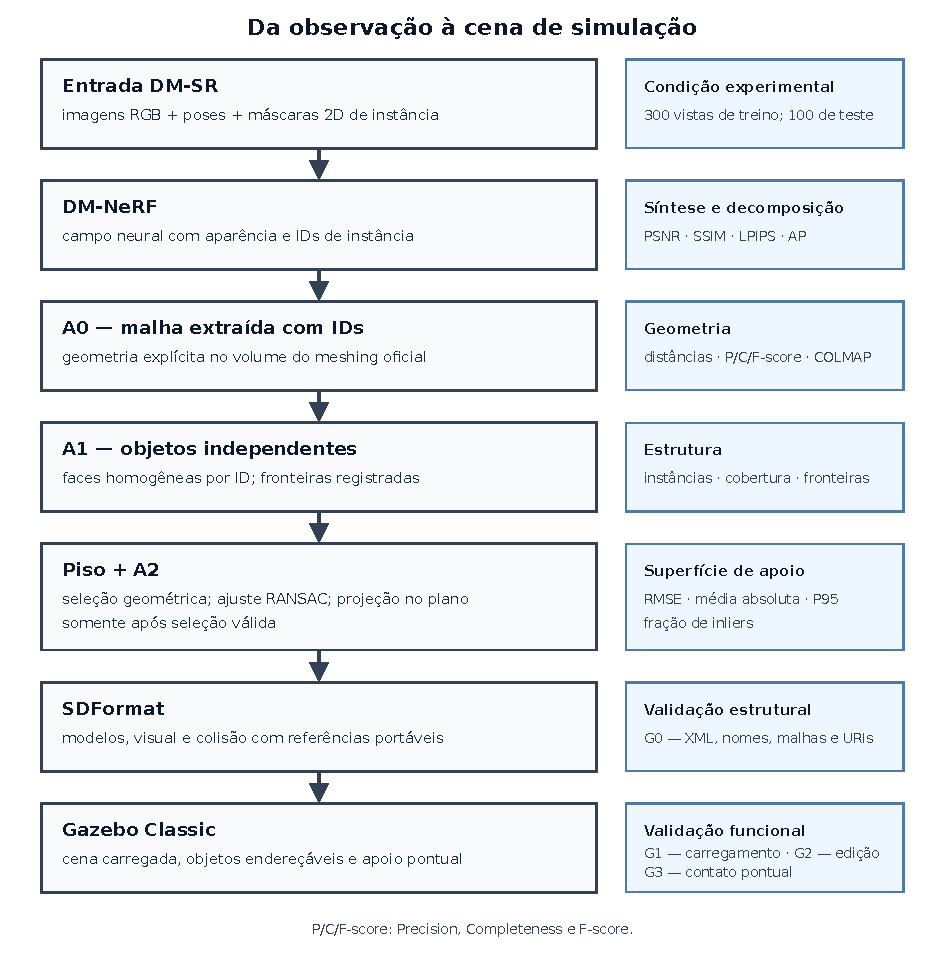
\includegraphics[width=0.90\textwidth]{method_pipeline.pdf}
  \caption{Cadeia metodológica entre as observações do DM-SR e a cena no Gazebo Classic, com as medidas empregadas em cada etapa.}
  \label{fig:method_pipeline}
\end{figure}

Por convenção deste experimento, as condições da ablação interna são identificadas pelo prefixo A: A0 corresponde à malha extraída, A1 acrescenta a separação dos objetos e A2 acrescenta a regularização do piso. As verificações no Gazebo recebem o prefixo G e avançam da validação estática, G0, aos ensaios funcionais G1--G3. A numeração expressa, portanto, a progressão cumulativa da cadeia, e não uma nomenclatura própria do DM-NeRF.

As etapas e suas medidas são apresentadas na Tabela~\ref{tab:etapas}. A organização evita atribuir a uma etapa uma métrica que ela não pode alterar. A separação estrutural A1, por exemplo, não modifica intencionalmente as coordenadas das faces preservadas e, portanto, não é avaliada por PSNR ou por ganho de distância de superfície.

\begin{table}[H]
\centering
\small
\caption{Etapas da cadeia e medidas utilizadas.}
\label{tab:etapas}
\begin{tabularx}{\textwidth}{p{2.1cm}Y Y}
\toprule
\textbf{Etapa} & \textbf{Transformação} & \textbf{Medida principal} \\
\midrule
Neural & treinamento e avaliação do DM-NeRF & PSNR, SSIM, LPIPS e AP em vistas de teste \\
A0 -- malha & extração da malha & distâncias de superfície, Precision, Completeness e F-score \\
A1 -- objetos & separação por IDs explícitos & número de instâncias, cobertura de faces e fronteiras \\
A2 -- piso & regularização do candidato a piso & resíduos ao plano antes/depois \\
Gazebo & exportação e execução & verificações G0--G3 \\
\bottomrule
\end{tabularx}
\end{table}

\section{Conjunto de dados DM-SR}

O conjunto DM-SR fornece imagens RGB, poses de câmera, mapas bidimensionais de instância e uma malha tridimensional de referência. Para a cena \textit{study}, o experimento utiliza 300 imagens de treinamento e 100 vistas de teste do protocolo original. A malha de referência e os metadados de câmera são mantidos nas avaliações geométricas; quatro vistas de teste são usadas nas comparações qualitativas.

Quatro vistas reais da cena, extraídas do conjunto de teste, são apresentadas posteriormente junto às renderizações correspondentes do DM-NeRF (Figura~\ref{fig:render_comparison}). Essa comparação introduz visualmente a configuração doméstica/escritório e evita repetir as mesmas imagens em figuras distintas.

A malha de referência tem 437.008 vértices e 844.701 faces. O procedimento oficial de extração de malha do DM-NeRF utiliza o \textit{oriented bounding box} dessa referência para definir o volume e a orientação da consulta ao campo neural. Dessa forma, a referência participa da definição do domínio de extração, e as métricas geométricas são interpretadas dentro desse domínio.

Os mapas de instância do DM-SR utilizam identificadores inteiros, mas os artefatos inspecionados não fornecem um catálogo semântico completo que associe cada ID a uma classe do ambiente. Em particular, não foi encontrada uma associação oficial entre um ID e a classe piso.

\section{Treinamento e avaliação do DM-NeRF}

A reprodução utiliza a implementação oficial do DM-NeRF. A configuração final usa 64 amostras no passe inicial, 128 amostras adicionais, 3.072 raios no treinamento e 1.024 raios no avaliador. O treinamento foi realizado com precisão mista automática; a avaliação final e a extração da malha foram mantidas em FP32.

O avaliador oficial calcula a razão sinal-ruído de pico (PSNR), o índice de similaridade estrutural (SSIM) \citep{wang2004ssim} e a distância perceptual LPIPS \citep{zhang2018lpips} para síntese de vistas; o PSNR segue a definição usada no protocolo do DM-NeRF \citep{wang2023dmnerf}. Para decomposição, a interseção sobre união (IoU) mede a sobreposição entre uma máscara predita e sua referência, e a precisão média (AP) resume a qualidade das detecções em um limiar de IoU, conforme o avaliador do método. Valores maiores indicam melhor correspondência. São usados os limiares de IoU 0,50, 0,75, 0,80, 0,85, 0,90 e 0,95. A função de perda e as métricas emitidas durante o treinamento não são utilizadas como resultados de teste.

\section{Extração da malha e contrato de rótulos}

Após o treinamento, o campo neural é consultado no volume definido pelo procedimento oficial e convertido em malha triangular. A condição A0 reúne a geometria extraída e um vetor de identificadores de instância associado aos vértices. As cores presentes na visualização são usadas somente para apresentação; a separação estrutural consulta os identificadores explícitos, e não valores RGB.

Antes de separar objetos, o contrato verifica a quantidade e a ordem dos vértices, os índices dos triângulos, a topologia e a finitude das coordenadas. Essa verificação impede a associação de IDs a uma malha com ordem de vértices diferente. A malha final contém 356.272 vértices e 710.928 faces.

\section{Separação estrutural (A1)}

A condição A1 é formada a partir de A0. Para cada triângulo, são consultados os IDs de seus três vértices. Uma face é atribuída a uma instância somente quando os três IDs coincidem. Faces com IDs diferentes são classificadas como faces de fronteira e permanecem fora das malhas individuais. A decisão evita escolher arbitrariamente um dos rótulos presentes na face.

Para cada instância com faces homogêneas, os vértices utilizados são remapeados e uma malha independente é exportada. São registrados o ID, o número de vértices e faces, a área, os limites espaciais e o centroide. A cobertura de faces homogêneas e a quantidade de fronteiras são calculadas sobre a topologia original.

\section{Seleção geométrica do piso}

Como não há rótulo semântico oficial para o piso, a seleção usa uma heurística geométrica definida antes da observação da malha final. Cada instância é analisada somente pelas faces homogêneas. O plano principal é obtido por covariância dos vértices dessas faces com ponderação pela área dos triângulos. São calculados área, fração de área aproximadamente horizontal, normal, altura e RMSE do ajuste.

Uma instância é elegível quando satisfaz simultaneamente: área de pelo menos 0,5 m$^2$; pelo menos 85\% da área com orientação de até 15 graus da vertical; normal do plano dentro do mesmo limite angular; RMSE de no máximo 0,03 m; e posição na faixa inferior da cena, definida pelo percentil 1 das alturas acrescido de 20\% da amplitude vertical. O eixo vertical da malha é +Y.

Entre candidatas elegíveis, a maior área é escolhida se a segunda candidata tiver área inferior a 80\% da primeira. Caso contrário, a saída é ambígua. Se nenhuma instância for elegível, a saída é ``não identificada''. Em ambos os casos de abstenção, A2 é bloqueada. A regra não utiliza cor, número de ID ou associação histórica como critério semântico.

\section{Regularização do piso (A2)}

Quando existe candidato válido, os vértices associados ao ID selecionado são usados no algoritmo \textit{Random Sample Consensus} (RANSAC) de \citet{fischler1981ransac}, que ajusta um modelo robusto mesmo na presença de pontos discrepantes. O limiar é 2 cm e a semente é fixa. O plano final é ajustado aos inliers. A regularização projeta apenas os vértices da instância selecionada sobre esse plano. A topologia e os IDs não são alterados.

O efeito é medido sobre o mesmo subconjunto antes e depois da projeção. São reportados erro absoluto médio, RMSE, P95 e fração de inliers. Uma redução desses resíduos indica apenas maior aderência ao plano estimado. Como a operação é uma projeção, a redução é esperada por construção e não demonstra aumento de fidelidade global em relação ao ambiente real.

\section{Exportação para Gazebo Classic}

A exportação gera mundos SDFormat com referências relativas. A0 é representada por uma malha única. A1 e A2 são representadas por modelos independentes derivados das instâncias. Cada modelo possui um link, um elemento visual e um elemento de colisão apontando para a mesma malha triangular. O referencial +Y da reconstrução é rotacionado para +Z do Gazebo por uma transformação rígida comum.

A validação G0 verifica XML, nomes únicos, existência das malhas, caminhos relativos, escalas positivas e correspondência entre visual e colisão. Essa etapa não executa a física e não substitui o parser nativo do Gazebo. G1, G2 e G3 verificam, respectivamente, carregamento real, manipulação independente e suporte/colisão do piso.

\chapter{Protocolo experimental}\label{cap:protocolo}

\section{Unidade experimental e proveniência}

A cena \textit{study} é a unidade experimental. Ela representa um ambiente de trabalho com mesas, cadeiras, armário e objetos menores sobre o mobiliário. A Figura~\ref{fig:study_scene} apresenta uma vista RGB do próprio DM-SR, diferente das quatro vistas usadas posteriormente na comparação quantitativa. Essa imagem permite reconhecer os elementos cuja aparência, geometria e separação são avaliadas ao longo do protocolo.

\begin{figure}[H]
  \centering
  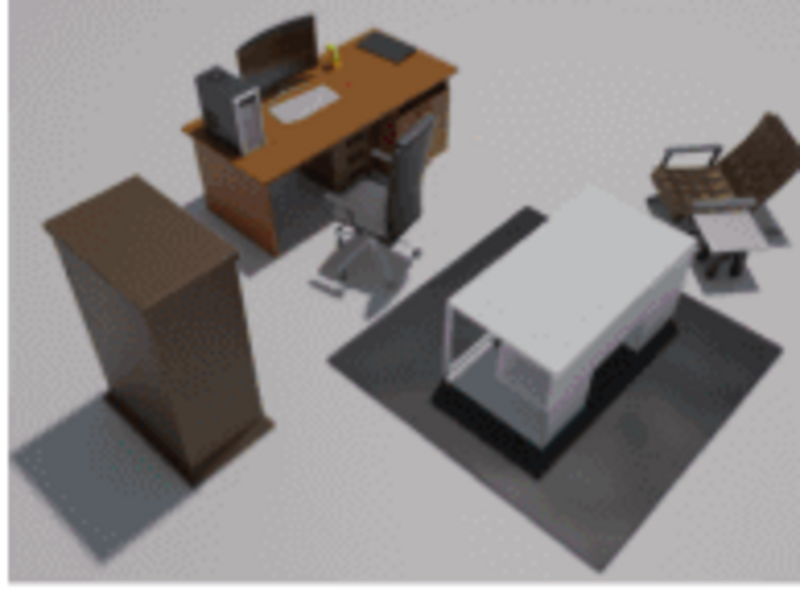
\includegraphics[width=0.60\textwidth]{study_scene_reference.png}
  \caption{Vista RGB de referência da cena \textit{study}, usada como estudo de caso. A cena contém duas mesas, assentos, armário e objetos menores; esses elementos aparecem posteriormente na avaliação da síntese, da geometria e da separação por instâncias. Fonte: material oficial do DM-NeRF/DM-SR \citep{wang2023dmnerf}.}
  \label{fig:study_scene}
\end{figure}

O mesmo modelo, obtido após 200.000 iterações em três sessões de treinamento, é empregado na avaliação de vistas, na decomposição e na extração geométrica. Ensaios preliminares de desempenho e infraestrutura não são incorporados aos resultados científicos.

A configuração, o ambiente computacional e as saídas brutas foram preservados para reprodução. Antes da análise, verificou-se a consistência entre o resumo do avaliador oficial, as métricas das 100 vistas de teste e os artefatos geométricos extraídos.

Os scripts, configurações e instruções de execução estão versionados no repositório \mbox{\url{https://github.com/Jfsslemos/sdf-generator}}. A configuração empregada nos resultados corresponde ao commit \texttt{e8bef9b7dc77}. O repositório registra o processamento desde o treinamento e a avaliação oficial até a extração, a separação por instância, a análise geométrica, a exportação SDFormat e os testes estáticos. As saídas numéricas usadas nas tabelas permanecem associadas aos arquivos que as produziram, enquanto artefatos volumosos são mantidos fora do controle de versão.

\section{Condições de ablação A0, A1 e A2}

O prefixo A identifica as condições da ablação interna, e a numeração representa estados cumulativos do pós-processamento: 0 para a saída sem essas transformações, 1 após a separação estrutural e 2 após a regularização do piso. As três condições são derivadas da mesma reconstrução:
\begin{itemize}
  \item \textbf{A0}: malha extraída do campo neural, antes do pós-processamento geométrico;
  \item \textbf{A1}: A0 separada em objetos por IDs explícitos de instância; e
  \item \textbf{A2}: A1 com projeção dos vértices do candidato a piso sobre o plano estimado.
\end{itemize}

A0 é avaliada por métricas de superfície. A1 é avaliada por cobertura da separação e quantidade de objetos; as coordenadas das faces preservadas não são modificadas. A2 é avaliada por métricas pareadas do piso e por suporte e colisão no simulador.

\section{Síntese de vistas e decomposição}

Esta etapa verifica duas propriedades do modelo treinado. A primeira é se ele gera, para câmeras de teste, imagens próximas às referências. A segunda é se o ID previsto em cada região da imagem corresponde ao objeto indicado pelo mapa de instâncias de referência.

As métricas de síntese são PSNR, SSIM e LPIPS. Para PSNR e SSIM, valores maiores indicam maior semelhança com a imagem de referência; para LPIPS, valores menores indicam maior semelhança perceptual. Na decomposição, a interseção sobre união (IoU) mede quanto a máscara prevista e a máscara de referência se sobrepõem. A precisão média (AP) resume as correspondências que atingem um limiar mínimo de IoU. São usados AP50, AP75, AP80, AP85, AP90 e AP95. Quanto maior o sufixo, mais exata precisa ser a sobreposição; em todos os casos, AP maior é melhor. As médias são calculadas sobre as 100 vistas de teste e conferidas contra os resultados individuais.

\section{Avaliação geométrica}

A avaliação geométrica verifica se a superfície reconstruída ocupa posições próximas às da malha de referência e se cobre as mesmas regiões da cena. Essa verificação é distinta da comparação de imagens: um objeto pode aparecer corretamente em uma vista e estar deslocado em profundidade.

A0 e a malha de referência são amostradas com 200.000 pontos de superfície, usando a semente 42 para tornar a amostragem repetível. Para cada ponto de A0, calcula-se a distância até o ponto mais próximo da referência; depois, repete-se o cálculo da referência para A0. As duas direções são necessárias porque uma reconstrução pode produzir pontos próximos da referência e, ao mesmo tempo, deixar regiões da referência sem cobertura. As métricas incluem a distância média em cada direção, a soma das duas médias como distância simétrica L1 e o RMSE em cada direção.

Para um limiar $t$, Precision é a fração dos pontos reconstruídos que está a no máximo $t$ da referência. Completeness é a fração dos pontos da referência que encontra algum ponto reconstruído a no máximo $t$. O F-score é a média harmônica dessas duas frações e só permanece alto quando precisão e cobertura são altas. O protocolo usa limiares de 1, 2 e 5 cm para mostrar como a conclusão muda entre uma exigência de coincidência fina e uma tolerância mais ampla.

A interpretação considera a dependência do bounding frame da referência no meshing oficial. Portanto, as métricas descrevem a saída dentro do protocolo reproduzido; não são apresentadas como uma avaliação cujo volume de extração foi obtido independentemente do \textit{ground truth}.

\section{Baseline geométrico externo}

O COLMAP reconstrói a geometria procurando pontos correspondentes em imagens obtidas de diferentes posições. Ele é usado somente como referência externa para a geometria: sua nuvem de pontos e a malha A0 são comparadas à mesma malha de referência. O COLMAP não participa da separação A1, da regularização A2 nem dos testes no Gazebo.

Foi executado o MVS denso do COLMAP \citep{schonberger2016mvs} com as 300 imagens de treinamento da cena \textit{study}. Nesse processo, o PatchMatch estima profundidades ao procurar correspondências entre imagens, e a fusão reúne os mapas de profundidade em uma nuvem. As poses e os intrínsecos oficiais do DM-SR foram fornecidos diretamente; portanto, o ensaio mede a reconstrução densa e não a capacidade do COLMAP de estimar as câmeras. Para cada imagem de referência foram selecionadas as dez câmeras mais próximas em posição. O PatchMatch utilizou consistência geométrica, intervalo de profundidade de 4 a 15 m, e a fusão foi executada com \texttt{min\_num\_pixels=1}. Não foi realizada busca de hiperparâmetros.

A saída do COLMAP permanece no sistema de coordenadas das poses do DM-SR, enquanto o gerador de malha do DM-NeRF consulta a rede após a permutação de eixos \([x,y,z]_{rede}=[x,-z,y]_{cena}\). Antes da comparação, a nuvem COLMAP é portanto convertida de volta para o sistema da malha por \([x,y,z]_{cena}=[x,z,-y]_{COLMAP}\).

Há ainda uma diferença na região espacial coberta por cada saída. O meshing oficial do DM-NeRF consulta somente uma caixa orientada definida a partir da referência, com extensões fixas de \(1,9\times7,0\times7,0\) m, enquanto o COLMAP pode produzir pontos além dessa caixa. Comparar volumes diferentes poderia penalizar o COLMAP apenas por reconstruir uma região maior ou favorecer um método por avaliar uma região menor. Por isso, as duas saídas são medidas no mesmo suporte orientado. Dos 5.800.316 pontos fundidos pelo COLMAP, 3.416.962 (58,91\%) permanecem dentro desse volume. Em seguida, 200.000 pontos são amostrados com semente 42, igualando a cardinalidade usada na avaliação de A0. As métricas são calculadas pelas mesmas definições de distância, Precision, Completeness e F-score.

Os números produzidos diretamente pelo notebook antes dessa conversão de coordenadas e da equalização de suporte não são usados na análise comparativa, pois misturam convenções de referência distintas.

\section{Avaliação da separação e do piso}

A avaliação de A1 verifica se os IDs associados aos vértices podem ser convertidos em objetos independentes sem modificar a posição das faces preservadas. São registrados o número de instâncias, as faces homogêneas, as faces de fronteira e a cobertura. As faces de fronteira permanecem contabilizadas mesmo quando são omitidas das malhas individuais.

Para o piso, o relatório registra todos os candidatos e os motivos de rejeição. O RANSAC, ou consenso de amostras aleatórias, estima um plano a partir de subconjuntos de pontos e escolhe o modelo sustentado pelo maior conjunto de pontos próximos. A regularização usa limiar de 2 cm, 2.000 iterações e semente 42. O P95 é mantido como medida principal, acompanhado de média absoluta, RMSE e fração de inliers.

\section{Validação funcional}

O prefixo G identifica as verificações realizadas no Gazebo. A numeração avança da verificação estrutural estática para ensaios funcionais progressivamente mais específicos:
\begin{description}
  \item[G0] validação estática do arquivo SDFormat e de suas referências;
  \item[G1] carregamento do mundo no Gazebo Classic sem erro fatal associado aos modelos;
  \item[G2] transformação independente de pelo menos uma instância em A1/A2;
  \item[G3] verificação pontual de apoio e colisão da superfície regularizada em A2.
\end{description}

G0 não é interpretado como demonstração de comportamento físico. G1--G3 verificam, em sequência, carregamento, independência estrutural e contato no ponto ensaiado.

\section{Custo computacional}

São reportados tempo de treinamento, atualizações efetivas, atualizações puladas pelo AMP, pico de memória alocada pelo PyTorch, pico observado pela telemetria, tempo de avaliação e tempo de extração da malha. O uso de GPU gratuita é uma condição de reprodução, não uma métrica de qualidade.

\chapter{Resultados}\label{cap:resultados}

\section{Treinamento e custo computacional}

O treinamento foi concluído em três sessões, totalizando aproximadamente 30 h 58 min. O estado final registra 200.000 iterações, 199.916 atualizações efetivamente aplicadas pelo otimizador e 85 atualizações puladas pelo escalonador de AMP. Isso corresponde a aproximadamente 0,0425\% das tentativas de atualização. A diferença entre iterações e atualizações ocorre quando a precisão mista detecta valores numéricos inadequados e evita aplicar aquela atualização.

O pico de memória alocada pelo PyTorch foi de aproximadamente 5,58 GiB e o pico observado pela telemetria do dispositivo foi 7.417 MiB. A avaliação oficial levou 2.568,48 s (42,8 min) e a extração da malha levou 109,13 s (1,82 min). A Tabela~\ref{tab:custo} reúne esses valores.

\begin{table}[H]
\centering
\caption{Resumo da execução final.}
\label{tab:custo}
\begin{tabular}{lr}
\toprule
\textbf{Medida} & \textbf{Valor} \\
\midrule
Iteração final & 200.000 \\
Atualizações efetivas & 199.916 \\
Atualizações puladas por AMP & 85 \\
Tempo de treinamento & 30 h 58 min \\
Pico PyTorch & 5,58 GiB \\
Pico da telemetria & 7.417 MiB \\
Tempo de avaliação & 2.568,48 s \\
Tempo de meshing & 109,13 s \\
\bottomrule
\end{tabular}
\end{table}

A Tabela~\ref{tab:custo} mostra que o custo se concentra no treinamento por cena: avaliação e extração da malha somaram menos de 45 minutos, enquanto o treinamento consumiu quase 31 horas. Nesse regime, a cadeia prepara previamente um ambiente para simulação; ela não reconstrói a cena durante a execução de uma tarefa robótica.

\section{Síntese de vistas}

A Tabela~\ref{tab:metricas_neurais} reúne as médias do avaliador oficial sobre 100 vistas de teste. As três primeiras colunas medem a aparência das imagens: PSNR e SSIM aumentam com a semelhança à referência, enquanto LPIPS diminui quando a distância perceptual é menor. As seis colunas seguintes medem a correspondência das máscaras de instância em exigências crescentes de sobreposição. A média oficial coincide com a agregação dos resultados por vista. Os valores de imagem descrevem a projeção observada pelas câmeras, mas não medem a posição da superfície tridimensional.

\begin{table}[H]
\centering
\small
\caption{Métricas do avaliador oficial na cena \textit{study}.}
\label{tab:metricas_neurais}
\begin{tabular}{rrrrrrrrr}
\toprule
PSNR & SSIM & LPIPS & AP50 & AP75 & AP80 & AP85 & AP90 & AP95 \\
\midrule
41,1100 & 0,9875 & 0,0260 & 0,9956 & 0,9911 & 0,9849 & 0,9769 & 0,9311 & 0,7192 \\
\bottomrule
\end{tabular}
\end{table}

\subsection{Comparação com os resultados publicados do DM-NeRF}

A reprodução pode ser comparada diretamente aos valores publicados por \citet{wang2023dmnerf} para a mesma cena \textit{study} do DM-SR. Essa comparação é distinta de um novo baseline: seu objetivo é verificar se o estágio neural reproduz o comportamento reportado pelo método de origem antes de analisar as transformações propostas nesta dissertação. A Tabela~\ref{tab:repro_dmnerf} apresenta os valores.

\begin{table}[H]
\centering
\small
\caption{Comparação entre a reprodução desta dissertação e os resultados publicados para a cena \textit{study} do DM-SR.}
\label{tab:repro_dmnerf}
\begin{tabular}{lrrrr}
\toprule
\textbf{Fonte} & \textbf{PSNR (dB)} & \textbf{SSIM} & \textbf{LPIPS} & \textbf{AP$_{0,75}$ (\%)} \\
\midrule
Wang et al. (2023) & 41,08 & 0,987 & 0,026 & 98,86 \\
Esta reprodução & 41,110 & 0,9875 & 0,0260 & 99,11 \\
\bottomrule
\end{tabular}
\end{table}

As diferenças são de 0,03 dB em PSNR, 0,0005 em SSIM, aproximadamente zero em LPIPS na precisão reportada e 0,25 ponto percentual em AP$_{0,75}$. Como PSNR, SSIM e AP aumentam com a qualidade e LPIPS diminui, a proximidade ocorre em todas as direções esperadas das métricas. Com uma única cena, esses desvios não sustentam uma análise de significância estatística; eles mostram que a execução reproduz proximamente os valores publicados para \textit{study}.

O mesmo artigo reporta, para a cena \textit{study}, AP$_{0,75}$ de 96,86\% para Mask R-CNN e 97,88\% para Swin Transformer, ambos ajustados por cena, contra 98,86\% do DM-NeRF publicado. A reprodução desta dissertação obteve 99,11\%. Em relação aos valores publicados dos dois baselines 2D, a diferença é de 2,25 e 1,23 pontos percentuais, respectivamente. Esses números são usados como referência de literatura e não como reexecução independente dos baselines.

A Figura~\ref{fig:render_comparison} compara as vistas 0, 33, 66 e 99 com as renderizações correspondentes. Cada coluna deve ser lida verticalmente: a primeira linha é a referência, a segunda é a imagem gerada pelo DM-NeRF e a terceira marca a diferença absoluta. Como as duas primeiras linhas são visualmente próximas, a diferença foi ampliada por um fator cinco apenas para visualização. As áreas claras nessa terceira linha se concentram em contornos, sombras e detalhes do mobiliário, enquanto as superfícies maiores mantêm aparência semelhante.

\begin{figure}[H]
  \centering
  \begin{minipage}{0.88\textwidth}
    \centering
    \small (a) Referência DM-SR\par\vspace{0.25em}
    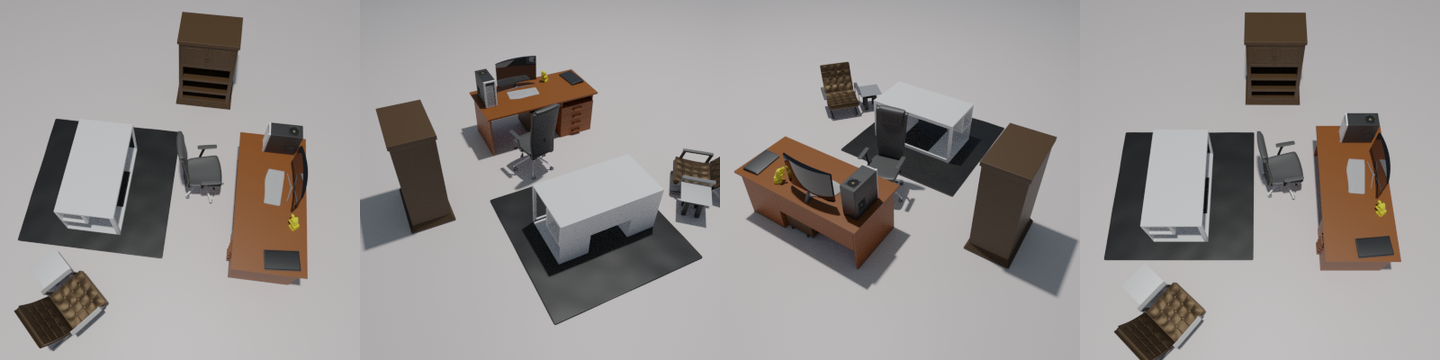
\includegraphics[width=\linewidth]{render_reference_row.png}\par\vspace{0.65em}
    \small (b) Renderização DM-NeRF\par\vspace{0.25em}
    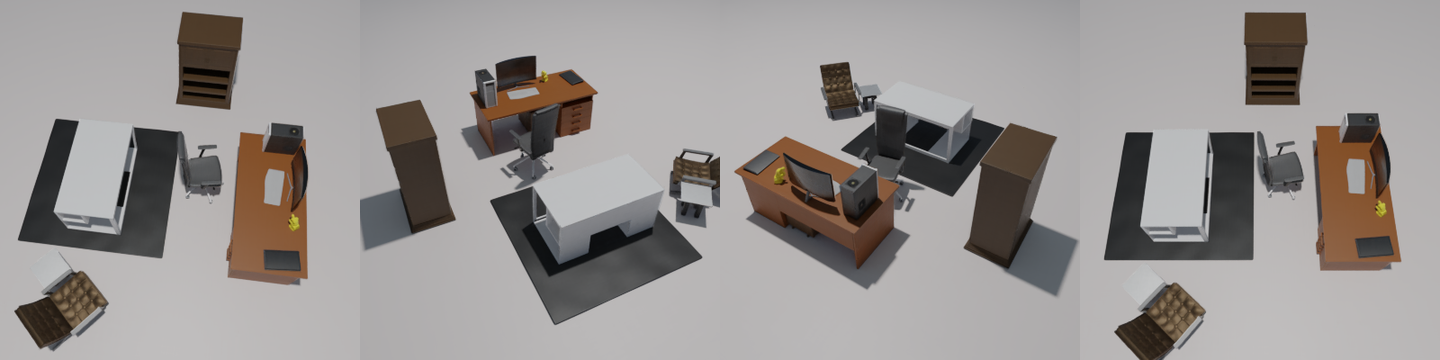
\includegraphics[width=\linewidth]{render_prediction_row.png}\par\vspace{0.65em}
    \small (c) Diferença absoluta ampliada $5\times$\par\vspace{0.25em}
    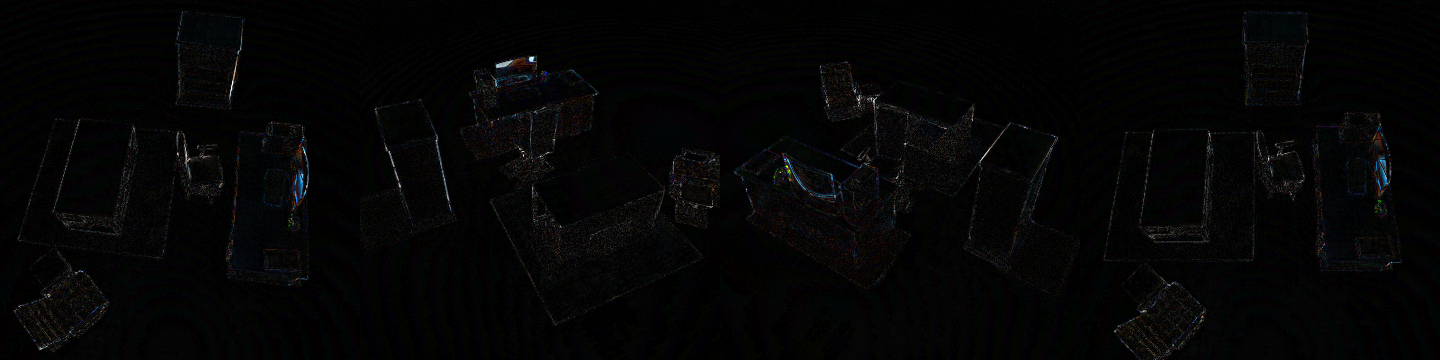
\includegraphics[width=\linewidth]{render_difference_row.png}
  \end{minipage}
  \caption{Síntese de vistas nas posições 0, 33, 66 e 99. A ampliação da diferença em (c) torna visíveis discrepâncias locais sem alterar as imagens comparadas.}
  \label{fig:render_comparison}
\end{figure}

\section{Decomposição de instâncias}

Os APs, para os quais valores maiores indicam melhor detecção e correspondência das máscaras, permanecem próximos de 1,0 nos limiares de IoU menos restritivos e diminuem quando a coincidência exigida se aproxima de 0,95. O AP50 é 0,9956, enquanto o AP95 é 0,7192. Esse comportamento indica que a correspondência geral das instâncias é mantida na maior parte das vistas, mas diferenças de contorno e pequenas regiões passam a afetar a métrica no limiar mais estrito. Como o protocolo fornece máscaras 2D durante o treinamento, os valores não demonstram descoberta de instâncias sem supervisão.

A Figura~\ref{fig:instancias_2d} compara os mapas de referência e predição nas mesmas quatro vistas. Cada cor identifica um objeto individual, e não sua categoria. A terceira linha marca em magenta os pixels cujo ID difere entre os dois mapas. O leitor deve observar que as regiões centrais dos objetos permanecem em grande parte iguais, enquanto as discordâncias se concentram nas fronteiras e em estruturas pequenas. Isso explica por que o AP permanece alto em IoU 0,50 e diminui quando a sobreposição exigida chega a 0,95.

\begin{figure}[H]
  \centering
  \begin{minipage}{0.88\textwidth}
    \centering
    \small (a) IDs de referência\par\vspace{0.25em}
    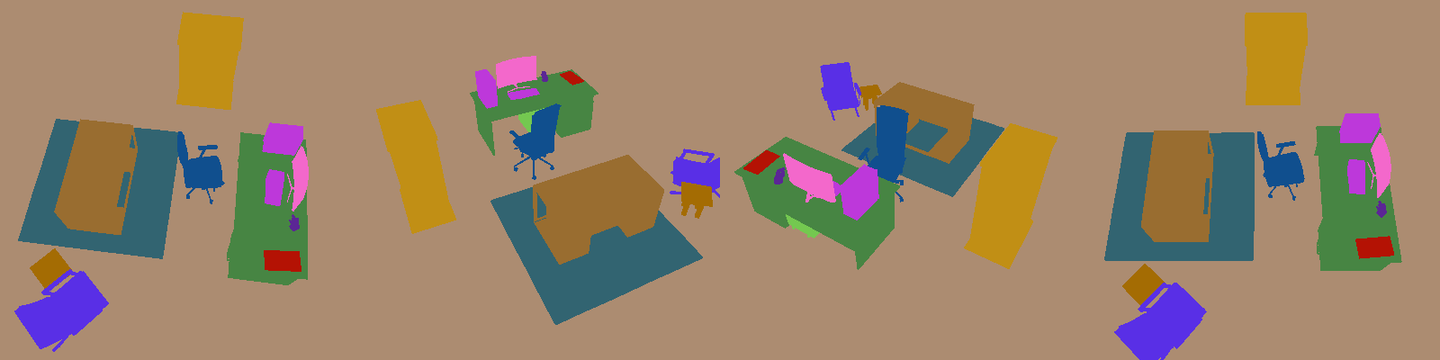
\includegraphics[width=\linewidth]{instance_reference_row.png}\par\vspace{0.65em}
    \small (b) IDs preditos pelo DM-NeRF\par\vspace{0.25em}
    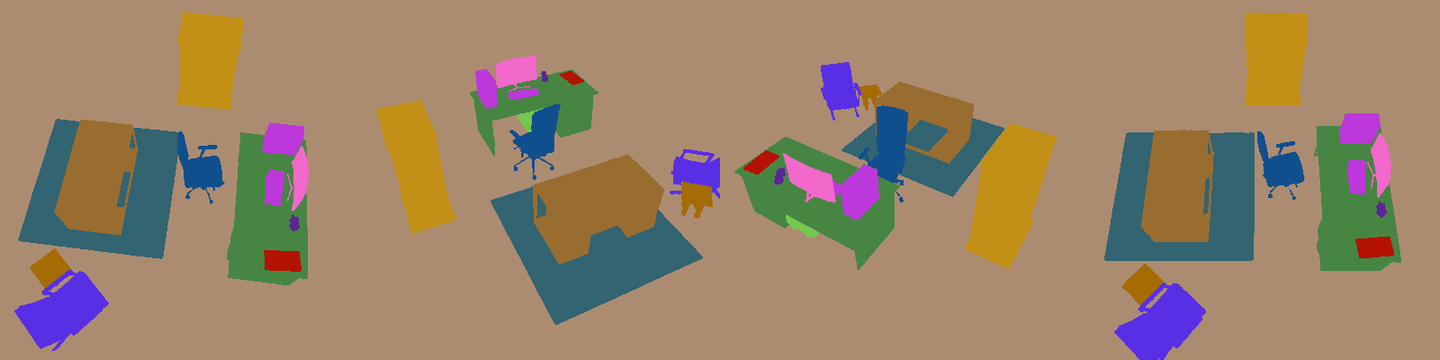
\includegraphics[width=\linewidth]{instance_prediction_row.png}\par\vspace{0.65em}
    \small (c) Pixels com IDs divergentes\par\vspace{0.25em}
    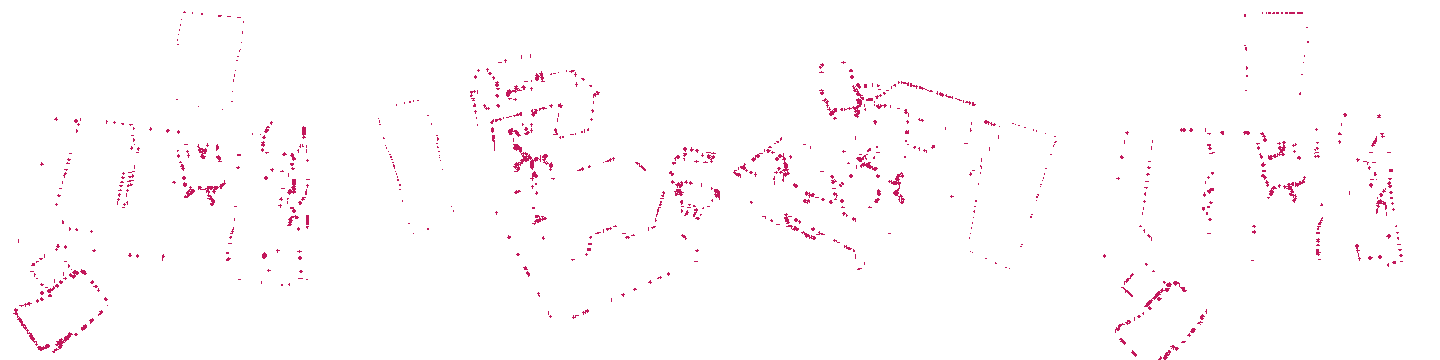
\includegraphics[width=\linewidth]{instance_difference_row.png}
  \end{minipage}
  \caption{Decomposição de instâncias nas vistas 0, 33, 66 e 99. Em (a) e (b), as cores identificam IDs, não classes semânticas; em (c), magenta indica divergência entre referência e predição.}
  \label{fig:instancias_2d}
\end{figure}

\section{Geometria extraída (A0)}

A malha A0 final contém 356.272 vértices e 710.928 faces. A comparação visual com a referência DM-SR e o COLMAP aparece na Figura~\ref{fig:geom_qual}, sem repetir o mesmo enquadramento em uma figura isolada. A estrutura global da sala e dos objetos principais é reconhecível, mas a visualização também mostra regiões ruidosas e superfícies que não formam volumes fechados.

A Tabela~\ref{tab:geom_dist} apresenta as distâncias médias e RMSE; em todas essas medidas, valores menores indicam maior proximidade entre as superfícies. As duas direções têm valores próximos: 4,34 cm da predição para a referência e 4,14 cm da referência para a predição. Essa proximidade entre as direções indica que o erro médio não é dominado apenas por pontos excedentes da reconstrução nem apenas por regiões ausentes da referência. Os RMSEs, maiores que as médias, mostram que alguns pontos estão mais afastados e recebem peso maior pelo erro quadrático.

\begin{table}[H]
\centering
\caption{Distâncias entre A0 e a referência DM-SR.}
\label{tab:geom_dist}
\begin{tabular}{lr}
\toprule
\textbf{Medida} & \textbf{Valor} \\
\midrule
Média predição $\rightarrow$ referência & 4,335 cm \\
Média referência $\rightarrow$ predição & 4,139 cm \\
Distância simétrica L1 & 8,474 cm \\
RMSE predição $\rightarrow$ referência & 5,757 cm \\
RMSE referência $\rightarrow$ predição & 4,940 cm \\
\bottomrule
\end{tabular}
\end{table}

Os resultados por limiar são apresentados na Tabela~\ref{tab:geom_threshold}. Precision mede a fração da reconstrução situada perto da referência; Completeness mede a fração da referência coberta pela reconstrução; e o F-score combina as duas medidas. Valores maiores são melhores. A 1 cm, somente cerca de 5\% dos pontos em cada direção encontram correspondência dentro do limiar. A 5 cm, Precision e Completeness passam de 0,75 e o F-score chega a 0,7750. Assim, a reconstrução representa melhor a estrutura quando se admite tolerância de 5 cm, sem sustentar coincidência fina em 1 cm.

\begin{table}[H]
\centering
\caption{Precision, Completeness e F-score da geometria A0.}
\label{tab:geom_threshold}
\begin{tabular}{rrrr}
\toprule
\textbf{Limiar} & \textbf{Precision} & \textbf{Completeness} & \textbf{F-score} \\
\midrule
1 cm & 0,04887 & 0,04724 & 0,04804 \\
2 cm & 0,20977 & 0,18398 & 0,19603 \\
5 cm & 0,79630 & 0,75478 & 0,77498 \\
\bottomrule
\end{tabular}
\end{table}

\section{Baseline geométrico externo: COLMAP}

O baseline COLMAP concluiu o PatchMatch e a fusão densa para as 300 vistas de treinamento, produzindo 5.800.316 pontos. Após a conversão para o sistema de coordenadas da malha e a restrição ao mesmo volume orientado empregado pelo meshing do DM-NeRF, 3.416.962 pontos permaneceram no suporte comum. A comparação usa uma amostra determinística de 200.000 pontos dessa nuvem, de modo a manter a mesma cardinalidade de A0 e da referência.

A Tabela~\ref{tab:colmap_geom} compara as duas reconstruções. A0 apresenta menor erro nas duas direções. A distância média da predição para a referência é 4,34 cm em A0 e 20,42 cm no COLMAP; no sentido referência para predição, os valores são 4,14 cm e 8,13 cm. A diferença entre as direções no COLMAP indica que parte relevante da superfície de referência possui pontos próximos, mas a nuvem contém espessamento e pontos afastados da superfície correta.

\begin{table}[H]
\centering
\small
\caption{Comparação geométrica entre A0 e o baseline COLMAP no mesmo suporte e com 200.000 pontos por conjunto.}
\label{tab:colmap_geom}
\begin{tabular}{lrr}
\toprule
\textbf{Medida} & \textbf{DM-NeRF A0} & \textbf{COLMAP} \\
\midrule
Média predição $\rightarrow$ referência & 4,335 cm & 20,418 cm \\
Média referência $\rightarrow$ predição & 4,139 cm & 8,129 cm \\
Distância simétrica L1 & 8,474 cm & 28,547 cm \\
RMSE predição $\rightarrow$ referência & 5,757 cm & 30,079 cm \\
RMSE referência $\rightarrow$ predição & 4,940 cm & 13,942 cm \\
\midrule
F-score a 1 cm & 0,0480 & 0,0285 \\
F-score a 2 cm & 0,1960 & 0,1288 \\
F-score a 5 cm & 0,7750 & 0,3721 \\
\bottomrule
\end{tabular}
\end{table}

A decomposição de Precision e Completeness ajuda a interpretar a diferença a 5 cm: A0 obtém 0,7963 e 0,7548, respectivamente, enquanto o COLMAP obtém 0,2710 e 0,5936. A completude do COLMAP é maior que sua precisão. Isso significa que sua nuvem chega perto de parte relevante da referência, mas uma parcela maior dos pontos reconstruídos permanece afastada da superfície correta. A Figura~\ref{fig:geom_qual} permite observar esse espessamento ao comparar as três colunas no mesmo enquadramento. A Figura~\ref{fig:geom_fscore} mostra, para ambos os métodos, o aumento do F-score quando a tolerância passa de 1 para 5 cm; barras maiores são melhores.

\begin{figure}[H]
  \centering
  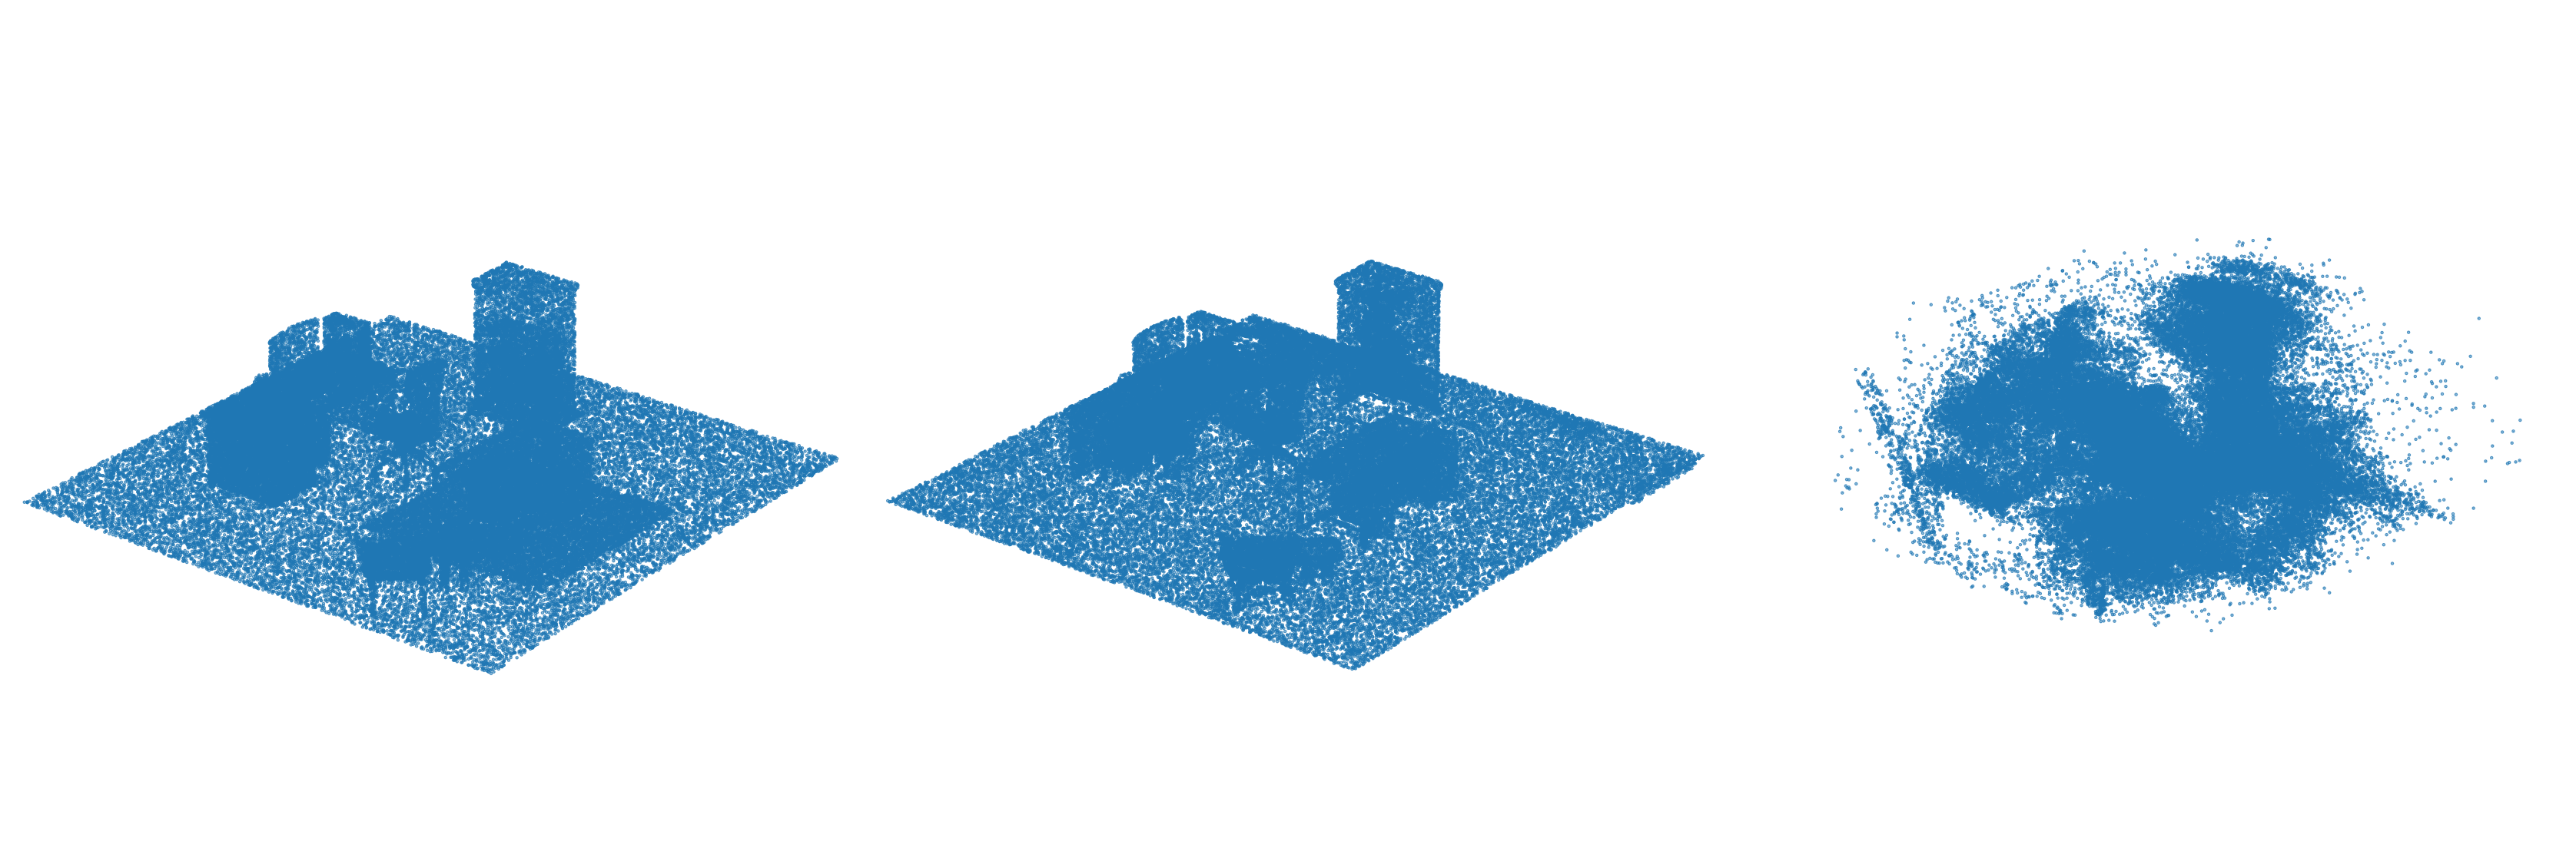
\includegraphics[width=\textwidth]{geometry_qualitative_comparison.png}
  \parbox{0.32\textwidth}{\centering\small (a) Referência DM-SR}\hfill
  \parbox{0.32\textwidth}{\centering\small (b) DM-NeRF A0}\hfill
  \parbox{0.32\textwidth}{\centering\small (c) COLMAP}
  \caption{Comparação qualitativa da geometria no mesmo sistema de coordenadas, suporte e enquadramento. A nuvem COLMAP apresenta maior dispersão e superfícies mais espessas.}
  \label{fig:geom_qual}
\end{figure}

\begin{figure}[H]
  \centering
  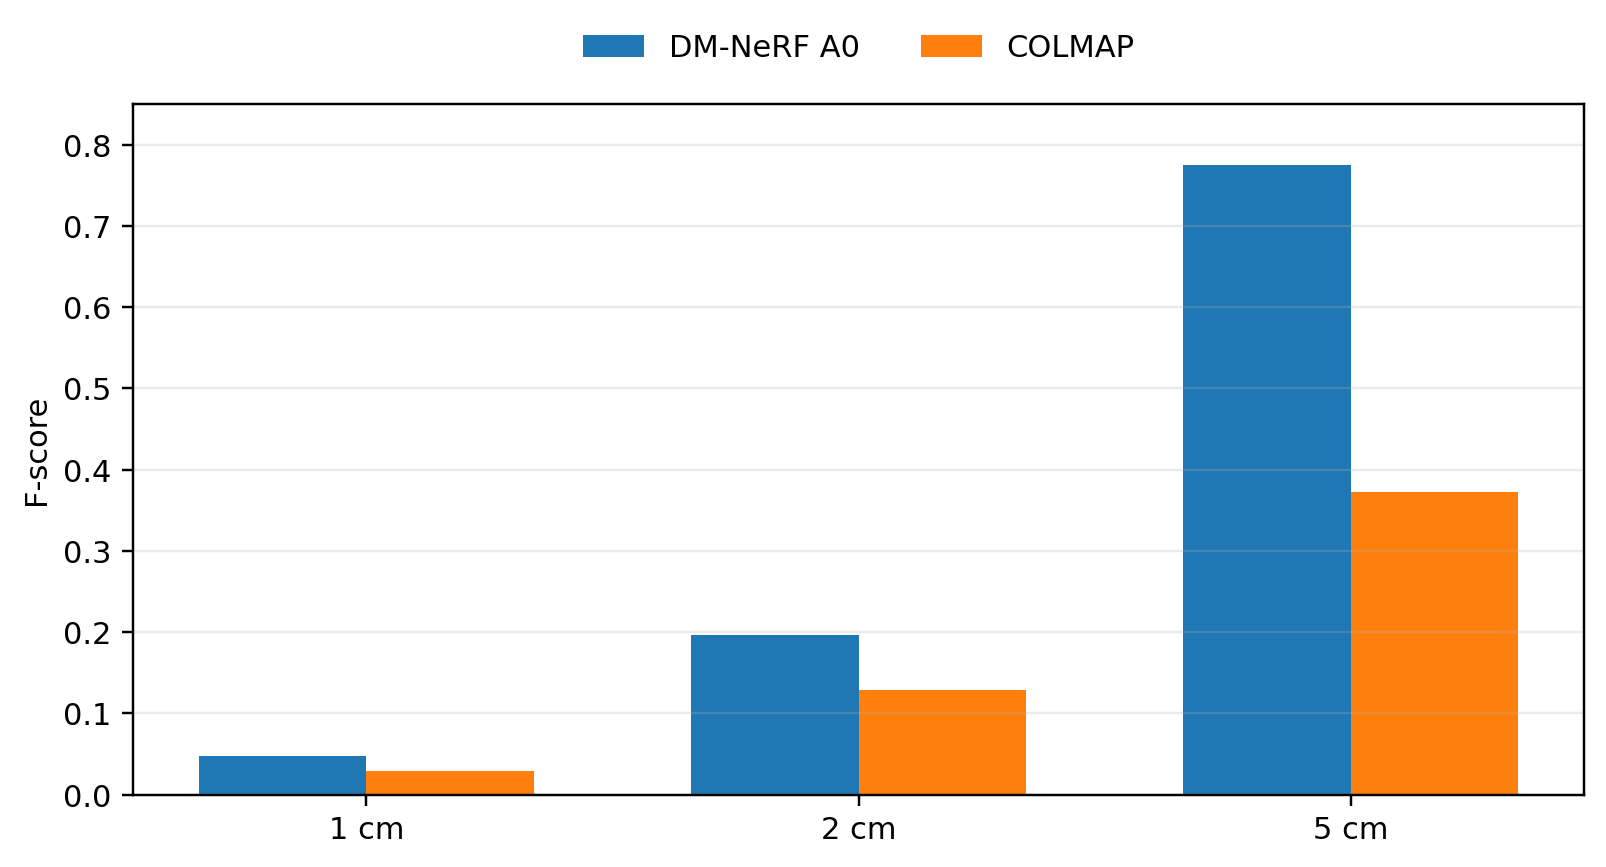
\includegraphics[width=0.82\textwidth]{geometry_fscore_comparison.png}
  \caption{F-score geométrico de A0 e COLMAP nos limiares de 1, 2 e 5 cm.}
  \label{fig:geom_fscore}
\end{figure}

\section{Separação estrutural (A1)}

A separação identificou 13 instâncias com faces homogêneas. Das 710.928 faces da malha original, 681.383 foram atribuídas a uma instância, enquanto 29.545 foram registradas como faces de fronteira. A Tabela~\ref{tab:a1} organiza essa contagem. A cobertura resultante é 95,844\%; nesse indicador, valores maiores representam maior preservação da topologia nas malhas individuais. A1 não melhora a geometria de A0: seu resultado é estrutural, pois transforma os IDs associados à malha em arquivos e modelos que podem ser manipulados separadamente. A cobertura não mede estanqueidade nem corrige erros geométricos da malha de origem.

\begin{table}[H]
\centering
\caption{Resumo da separação A1.}
\label{tab:a1}
\begin{tabular}{lr}
\toprule
Instâncias exportadas & 13 \\
Faces da malha A0 & 710.928 \\
Faces homogêneas exportadas & 681.383 \\
Faces de fronteira & 29.545 \\
Cobertura de faces homogêneas & 95,844\% \\
\bottomrule
\end{tabular}
\end{table}

A Figura~\ref{fig:a1} mostra a mesma reconstrução em dois pontos de vista. As mudanças de cor marcam as fronteiras entre IDs e permitem reconhecer quais partes se tornaram objetos distintos. A identidade empregada no processamento vem do vetor de IDs, não da cor armazenada em \texttt{mesh\_instances.ply}.

\begin{figure}[H]
  \centering
  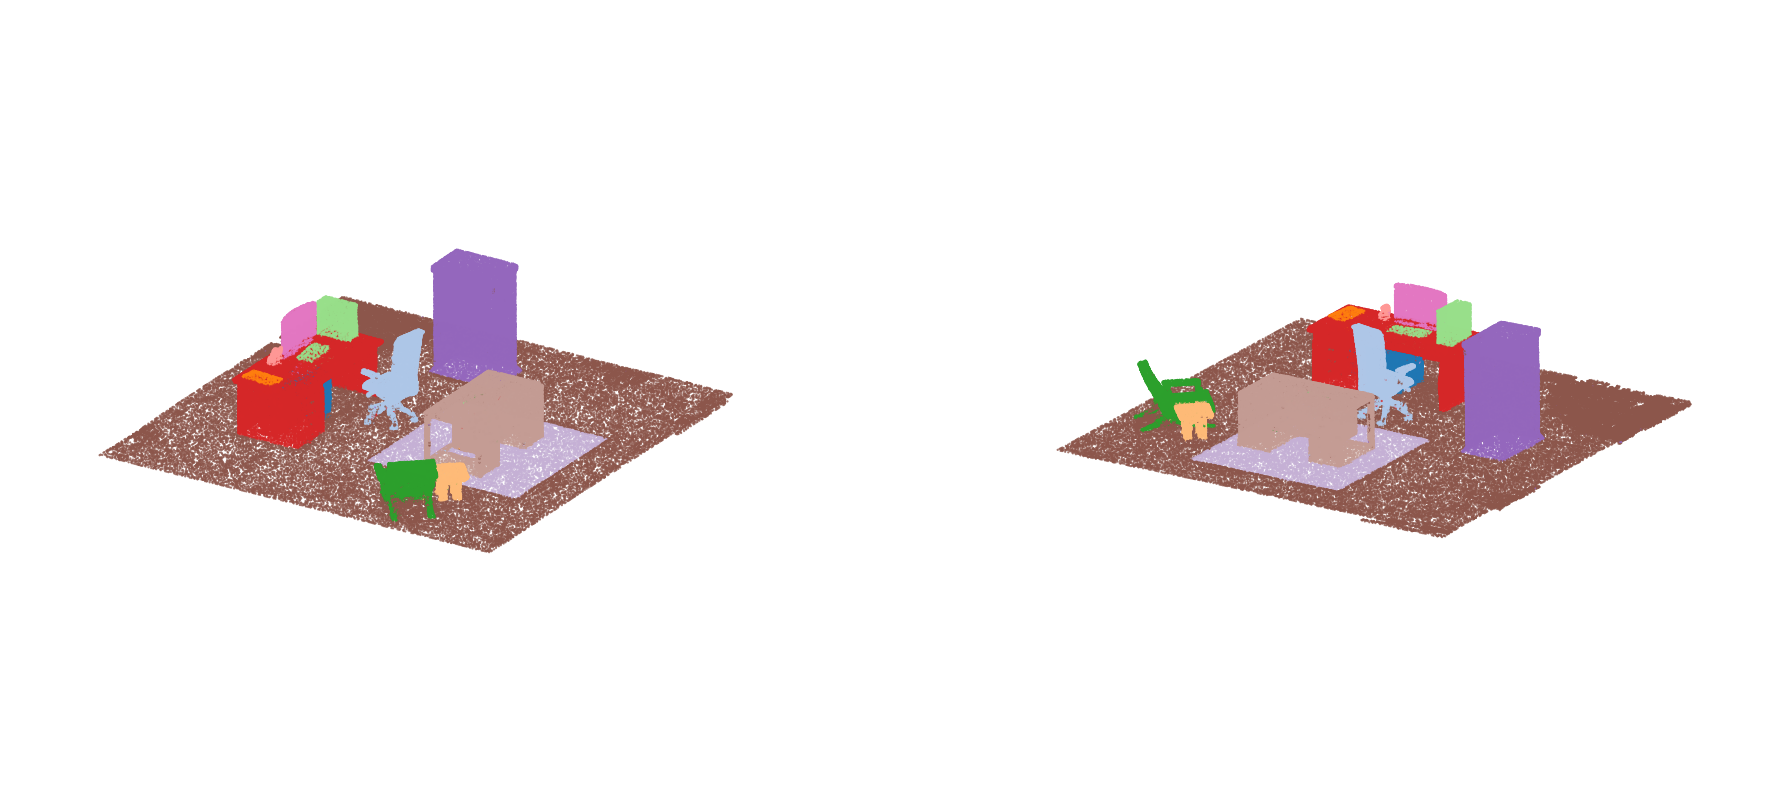
\includegraphics[width=\textwidth]{a1_instances.png}
  \caption{Visualização da reconstrução colorida por instância em dois pontos de vista. As cores são usadas somente para distinguir IDs.}
  \label{fig:a1}
\end{figure}

A individualização também foi verificada nos arquivos exportados por instância. Fragmentos e fronteiras permanecem visíveis em alguns objetos; por essa razão, a Figura~\ref{fig:a1} apresenta a cena completa colorida por ID, e a Figura~\ref{fig:gazebo_colorido} mostra posteriormente cada entidade carregada separadamente no Gazebo.

\section{Seleção e regularização do piso}

A heurística geométrica selecionou a instância 10. Ela foi a única instância a satisfazer simultaneamente os critérios de área, orientação, planaridade e altura. A instância 9 também apresenta grande fração horizontal e baixa altura, mas seu RMSE de 3,23 cm excede o limite de 3 cm definido antes da execução final. A seleção identifica um candidato geométrico e não constitui rótulo semântico de piso fornecido pelo DM-SR.

No RANSAC aplicado à instância selecionada, 77,11\% dos vértices ficaram a até 2 cm do plano estimado. Antes da projeção, a distância absoluta média era 2,051 cm, o RMSE era 5,722 cm e o P95 era 6,800 cm. O maior residual chegou a 1,64 m, indicando a presença de vértices associados ao mesmo ID afastados do plano principal. Esse valor não foi removido da análise.

A Tabela~\ref{tab:piso} compara o mesmo conjunto de vértices antes e depois da projeção. Para média absoluta, RMSE e P95, valores menores indicam maior proximidade ao plano; para a fração de inliers, valores maiores indicam que mais vértices estão a até 2 cm. A projeção de A2 leva os vértices selecionados ao plano, reduzindo média, RMSE e P95 a erro numérico. Essa redução ocorre por construção e descreve a planarização aplicada, não um aumento medido da fidelidade global da reconstrução. A consequência funcional é verificada separadamente pelo contato no Gazebo.

\begin{table}[H]
\centering
\caption{Métricas da instância 10 antes e depois da regularização.}
\label{tab:piso}
\begin{tabular}{lrr}
\toprule
\textbf{Medida} & \textbf{A1} & \textbf{A2} \\
\midrule
Média absoluta & 2,051 cm & $<10^{-12}$ cm \\
RMSE & 5,722 cm & $<10^{-12}$ cm \\
P95 & 6,800 cm & $<10^{-12}$ cm \\
Fração de inliers (2 cm) & 77,11\% & 100\% \\
\bottomrule
\end{tabular}
\end{table}

\begin{figure}[H]
  \centering
  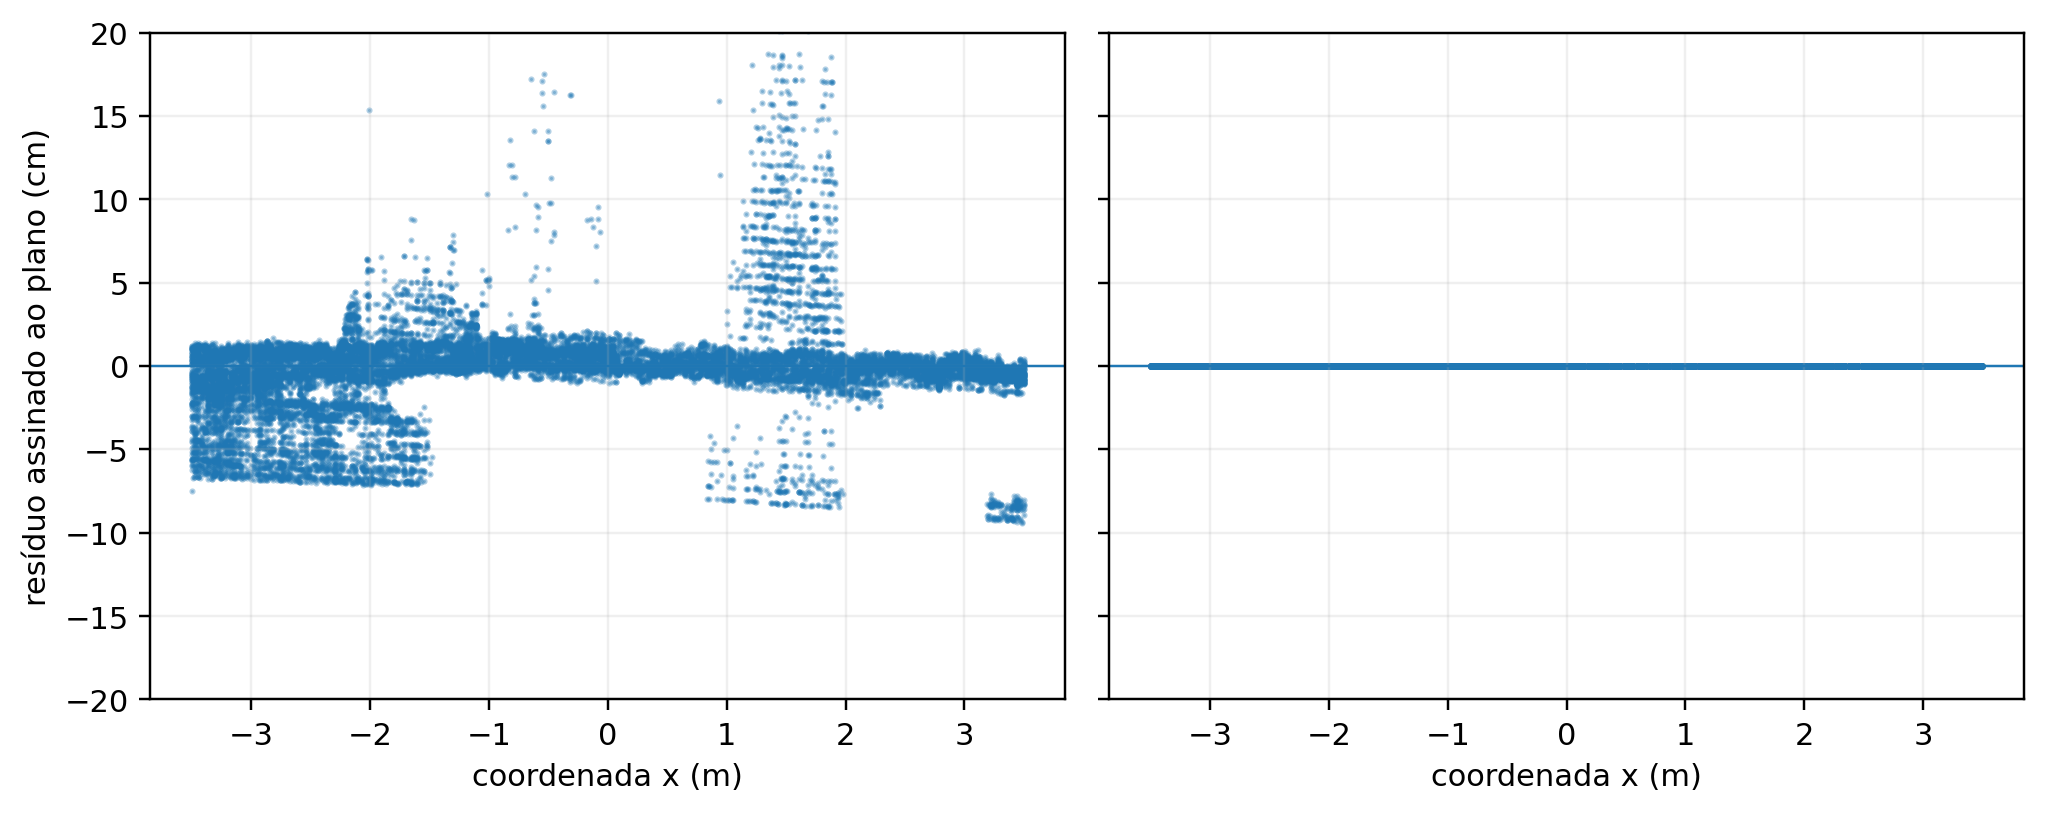
\includegraphics[width=\textwidth]{floor_residual_comparison.png}
  \caption{Resíduo assinado ao plano da instância 10 antes e depois da regularização. À esquerda, A1; à direita, A2. O eixo vertical é limitado a $\pm20$ cm para leitura da distribuição principal; o residual máximo de A1, 1,64 m, permanece reportado no texto e nas métricas.}
  \label{fig:piso}
\end{figure}

Na Figura~\ref{fig:piso}, a concentração dos pontos de A2 em torno de zero confirma o efeito da projeção. Em A1, a dispersão mostra as irregularidades do candidato original; o limite vertical de $\pm20$ cm permite ler a região principal sem ocultar do texto o residual máximo de 1,64 m.

\section{Integração no Gazebo Classic}

A Tabela~\ref{tab:gates} deve ser lida como uma sequência de propriedades distintas. G0 verifica a estrutura dos arquivos; G1 verifica se o Gazebo carrega os mundos; G2 verifica se um objeto separado pode ser deslocado sem mover os demais; e G3 verifica o contato em um ponto da superfície regularizada. A validação G0 passou para as três condições. A0 gerou um modelo correspondente à malha completa; A1 e A2 geraram 13 modelos independentes, com caminhos relativos para os arquivos de malha e correspondência entre os elementos visuais e de colisão.

Os testes de execução foram realizados no Gazebo Classic 11.10.2. Em G1, os mundos A0, A1 e A2 foram carregados e permaneceram ativos durante a janela de verificação. Foram observados apenas avisos relativos à aparência visual padrão, sem erros de carregamento das geometrias usadas nos testes.

Em G2, a instância \texttt{instance\_006} da condição A1 foi deslocada em 0,25 m no eixo $x$ por meio da interface do Gazebo. A pose consultada antes da operação era $(0,0,0)$ m e, após o comando, a coordenada $x$ passou para 0,25 m. A operação foi dirigida somente a esse modelo, demonstrando que a separação de A1 foi materializada em entidades endereçáveis de forma independente no simulador.

O teste G3 utilizou uma caixa dinâmica de 10 cm de lado e massa de 0,2 kg, posicionada com centro em $z=0,65$ m sobre uma região do candidato a piso regularizado. A primeira pose foi registrada seis segundos após o início da simulação, já depois da queda. Nesse instante, o centro da caixa estava em $z=0,093811$ m; oito segundos depois, estava em $z=0,093806$ m, variação de aproximadamente 5 $\mu$m.

Considerando metade da altura da caixa, sua face inferior permaneceu em $z=0,043806$ m. A altura calculada do plano regularizado no ponto $(x,y)=(3,07411,-3,31338)$ m, após a rotação comum de +Y para +Z usada na exportação, é $z=0,043810$ m. A diferença de aproximadamente 4 $\mu$m expressa a concordância numérica entre a pose registrada da face inferior da caixa e a altura calculada do plano no mesmo ponto, não uma medida de precisão física micrométrica do Gazebo. A caixa caiu aproximadamente 0,56 m, encontrou a superfície, não a atravessou no ponto ensaiado e permaneceu estável durante a segunda janela de observação; por esses critérios, G3 foi aprovado.

\begin{table}[H]
\centering
\caption{Resultado das verificações de integração com o Gazebo Classic.}
\label{tab:gates}
\begin{tabularx}{\textwidth}{>{\raggedright\arraybackslash}X c c c}
\toprule
\textbf{Verificação} & \textbf{A0} & \textbf{A1} & \textbf{A2} \\
\midrule
G0 -- validação estática & passou & passou & passou \\
G1 -- carregamento no Gazebo & passou & passou & passou \\
G2 -- manipulação independente & -- & passou & -- \\
G3 -- apoio/colisão do piso & -- & -- & passou \\
\bottomrule
\end{tabularx}
\end{table}

Para tornar a individualização visualmente verificável, a mesma cena A2 foi aberta com materiais de visualização distintos por instância. Essa alteração não modifica poses, geometrias de colisão nem os resultados G1--G3. Na Figura~\ref{fig:gazebo_colorido}, as cores diferentes mostram que os elementos foram carregados como modelos separados. A caixa vermelha no canto superior esquerdo corresponde ao corpo dinâmico usado no ensaio G3; sua presença permite localizar o teste pontual, mas a captura não mede por si só a qualidade do contato.

\begin{figure}[H]
  \centering
  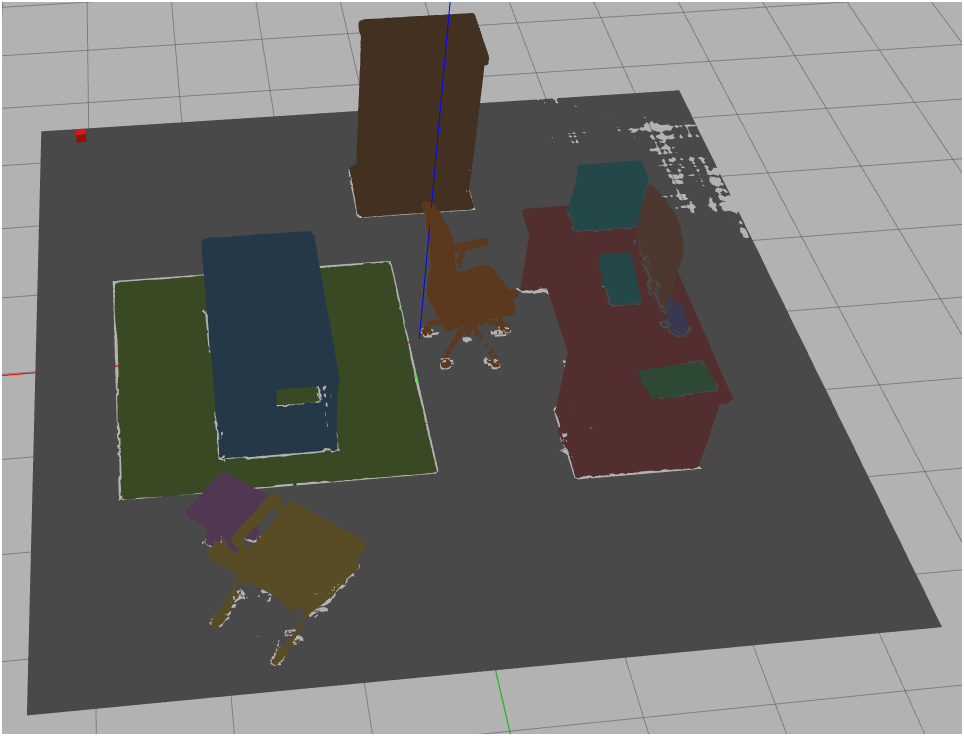
\includegraphics[width=0.88\textwidth]{gazebo_a2_colored.png}
  \caption{Cena A2 no Gazebo Classic com materiais visuais distintos por instância. As cores foram adicionadas somente para interpretação da figura; a geometria e as colisões são as mesmas usadas nos testes funcionais.}
  \label{fig:gazebo_colorido}
\end{figure}

\chapter{Discussão}\label{cap:discussao}

O principal resultado do experimento é a diferença entre qualidade de imagem e qualidade geométrica. O DM-NeRF reproduziu as vistas de teste da cena \textit{study} com métricas próximas às publicadas para a mesma cena, mas a correspondência da malha variou fortemente com a tolerância: o F-score passou de 0,0480 a 1 cm para 0,7750 a 5 cm. Assim, uma renderização próxima da referência não garante uma superfície adequada a contatos geométricos precisos. No mesmo suporte espacial, A0 obteve F-score superior ao COLMAP nos três limiares, sobretudo a 5 cm. Essa diferença caracteriza as configurações executadas, e não estabelece superioridade geral do DM-NeRF sobre MVS clássico.

A decomposição A1 demonstra que os IDs podem ser convertidos em objetos tridimensionais independentes. A regra conservadora preservou 95,844\% das faces homogêneas e manteve as faces de fronteira sem atribuição, evitando decidir arbitrariamente entre IDs conflitantes. Isso torna a separação auditável, mas pode produzir aberturas nas malhas. A seleção da instância 10 como piso também deve ser entendida como uma decisão geométrica, não como semântica fornecida pelo DM-SR. A projeção A2 regulariza a superfície de apoio por construção e atende a uma finalidade funcional; não constitui aumento demonstrado da fidelidade global.

Os testes no Gazebo confirmam carregamento, endereçamento independente de uma instância e contato no ponto ensaiado. Em G3, a caixa caiu, encontrou a superfície A2, não a atravessou e permaneceu estável na segunda observação. A concordância de aproximadamente 4 $\mu$m entre a pose registrada da face inferior e a altura calculada do plano não representa precisão física do simulador. Como o ensaio ocorreu em uma única posição e as malhas não são estanques, o resultado não caracteriza toda a superfície nem permite inferir propriedades físicas.

A contribuição da dissertação está, portanto, na avaliação da passagem de uma reconstrução DM-NeRF decomposta para geometria explícita, objetos independentes e uma cena utilizável no simulador, e não em uma nova arquitetura neural. Para a cena \textit{study}, essa passagem foi demonstrada sob o protocolo adotado, com perdas e hipóteses identificadas em cada estágio. A conclusão limita-se à cena e ao protocolo avaliados.

\chapter{Conclusão}\label{cap:conclusao}

Esta dissertação avaliou a transformação de uma reconstrução neural com decomposição de instâncias em uma representação explícita e estruturada para simulação robótica. A cadeia manteve o DM-NeRF como método neural e reuniu extração geométrica, individualização dos elementos, regularização de uma superfície de apoio e integração com o Gazebo Classic.

Na cena \textit{study}, a avaliação oficial em 100 vistas obteve PSNR de 41,1100 dB, SSIM de 0,9875 e LPIPS de 0,0260. A decomposição apresentou AP50 de 0,9956 e AP95 de 0,7192. A malha extraída atingiu F-score de 0,0480 a 1 cm, 0,1960 a 2 cm e 0,7750 a 5 cm, evidenciando a diferença entre qualidade de síntese e correspondência geométrica. No mesmo suporte, o COLMAP obteve 0,0285, 0,1288 e 0,3721 nesses limiares.

A separação estrutural gerou 13 objetos, preservou 95,844\% das faces homogêneas e registrou 29.545 faces de fronteira. A regra geométrica selecionou a instância 10 como superfície de apoio, e sua regularização reduziu o P95 do residual ao plano de 6,80 cm para erro numérico. Essas etapas estabeleceram uma correspondência explícita entre a topologia reconstruída, os identificadores de instância e os modelos exportados.

No Gazebo Classic, as três condições foram carregadas, uma instância foi manipulada de forma independente e a superfície regularizada sustentou o corpo dinâmico no ponto ensaiado. O protocolo distinguiu, assim, carregamento, independência estrutural e contato, em vez de tratar a simples abertura da malha no simulador como evidência suficiente.

Os resultados respondem afirmativamente à questão de pesquisa para a cena \textit{study} e o protocolo adotado: o pós-processamento transformou a reconstrução DM-NeRF em geometria explícita, objetos independentes e uma cena funcional no simulador. A contribuição do trabalho está na caracterização e avaliação dessa passagem, com evidências separadas para aparência, geometria, estrutura e funcionamento.


\bibliography{bibliografia}
\bibliographystyle{apalike}
\end{document}
